	\newcolumntype{P}[1]{>{\centering\arraybackslash}p{#1}} %para centralizar as colunas nas tabelas

	\thispagestyle{headfootimage}

\newpage
\FloatBarrier
\section{Identificação de áreas favoráveis para disposição final ambientalmente adequada}
\label{sec:areas_fav}
%% manual item II
%% Entrega 3: 26.nov.2019
%% Autora: Laís Shiki

A \gls{pnrs} (Lei n° 12.305/10) define que disposição ambientalmente adequada é a distribuição ordenada de rejeitos em aterros, observando normas operacionais específicas, como as normas ABNT NBR 13.896:1997 (Aterros de resíduos não perigosos - critérios para projeto, implantação e operação) e 15.849:2010 (Resíduos sólidos urbanos - Aterros sanitários de pequeno porte - Diretrizes para localização, projeto, implantação, operação e encerramento). Segundo essas normas, certos fatores devem ser analisados para a escolha da área a ser implantado o aterro, que são apresentados na \autoref{tab:fatores_aterro}.  

% Table generated by Excel2LaTeX from sheet 'fatores_aterro'
\begin{table}[htbp]
  \centering
  \caption{Fatores de análise para avaliação da área a ser implantado um aterro.}
    \begin{tabular}{P{40.955em}}
    \rowcolor[rgb]{ .992,  .914,  .851} \textbf{Tipo, consistência e granulometria das camadas de subsolo na base do aterro;} recomenda-se a utilização de solos naturalmente pouco permeáveis (solos argilosos, argilo-arenosos ou argilo-siltosos) \\
    \rowcolor[rgb]{ .984,  .831,  .706}\textbf{ No caso de existência de corpos d'água superficiais na área ou em entorno imdiato;} recomenda-se o respeito a uma distância mínima de 200 m de qualquer coleção hídrica ou curso d'água \\
    \rowcolor[rgb]{ .992,  .914,  .851} \textbf{Proximidade do freático em relação à base do aterro ou em seu entorno imediato} \\
    \rowcolor[rgb]{ .984,  .831,  .706} \textbf{Ocorrência de inundações:} as áreas com essas características não devem ser utilizadas \\
    \rowcolor[rgb]{ .992,  .914,  .851}\textbf{ Características topográficas da área devem ser tais que permitam uma das soluções adotáveis para o preenchimento do aterro,} recomenda-se locais com declividade superior a 1 \% e inferior a 30 \% \\
    \rowcolor[rgb]{ .984,  .831,  .706}\textbf{ Recomenda-se distância do limite da área útil do aterro a núcleos populacionais vizinhos mínima de 500 m} \\
    \rowcolor[rgb]{ .992,  .914,  .851} \textbf{Vida útil previsível do aterro sanitário de pequeno porte passível de ser implantado na área deve ser superior a 15 anos} \\
    \end{tabular}%
  \label{tab:fatores_aterro}%
  \legend{Fonte: \cite{abnt:13896}.}
\end{table}%

\FloatBarrier

Como foi discutido no Produto 2 deste \gls{pmgirs}, Monteiro Lobato está localizado nas escarpas e reversos da Serra da Mantiqueira, apresentando uma topografia montanhosa. A declividade média da região varia entre 17-20°, sendo que em sua maioria, o município apresenta áreas bastante declivosas (>20°). As áreas que possuem declividades menores estão associadas às áreas de várzeas dos rios Buquira/Ferrão e Buquirinha, não sendo o ideal para a implantação de um aterro sanitário. 

O município possui em seu território parte de uma unidade de conservação de uso sustentável, a Área de Preservação Ambiental (APA) da Bacia do Rio Paraíba do Sul, além da Reserva Particular do Patrimônio Natural (RPPN) Sítio do Cantoneiro e Áreas Prioritárias de Conservação. Logo, grande parte do território possui ao menos uma dessas unidades que ajudam a conservar o que restou da vegetação original. 

Monteiro Lobato apresenta uma rede de drenagem densa, o que é possível observar através da Figura 15 do Produto 2, o que faz dos recursos hídricos um fator importante para a cidade. As normas recomendam uma distância mínima de 200 m de qualquer corpo hídrico para a instalação de um aterro. Portanto, levando em consideração todos os aspectos discorridos acima, as áreas para se implantar um aterro sanitário no município são mínimas e ao entender deste \gls{pmgirs} são inexistentes.

\newpage
\FloatBarrier
\section{Identificação das possibilidades de soluções consorciadas ou compartilhadas com outros municípios}
\label{sec:sol_cons}
%% Manual item III
%% Entrega 1: 30.nov.2019
%% Autora: Laís Shiki


A \gls{pnrs} estabelece que os municípios que optarem por soluções consorciadas intermunicipais para a gestão dos resíduos sólidos, seguindo as diretrizes da Lei Federal n° 11.107/2005 que regulamenta os consórcios públicos, terão prioridade no acesso aos recursos da União \cite{brasil:12305}. Porém, é necessário cautela na escolha dos municípios a serem estabelecidos tais contratos. Segundo o Manual de Referência para elaboração do \gls{pmgirs} da \gls{agevap}, deve-se considerar a proximidade entre os locais, a possibilidade de compartilhamento de pessoal técnico, equipamentos e infraestrutura e as formas de prevenção de riscos ambientais com a perspectiva de economia de escala \cite{agevap_manual_2019}.

\subsection{Etapas para criação de um consórcio público}

Segundo a \gls{cnm}, as seguintes etapas devem ser seguidas a fim de se estabelecer um consórcio público intermunicipal \cite{consorcio_publico}: 

\begin{itemize}
	\item \textbf{Identificar os interesses e problemas em comum -} para se realizar o levantamento das dificuldades e problemas, é recomendável que sejam feitas reuniões/audiências públicas contendo a presença de agentes públicos de ambos municípios, a sociedade civil e uma equipe de trabalho técnica multidisciplinar;   
	
	\item \textbf{Elaborar Estudos de Viabilidade -} a equipe técnica deverá levantar as maneiras adequadas para resolver as necessidades identificadas, os passos a serem seguidos, os prazos e custos para desenvolver tal solução consorciada;
	
	\item \textbf{Elaborar o Protocolo de Intenções -} de acordo com o Art. 4° da Lei Federal n° 11.107/2005, o Protocolo de Intenções deve conter:
	\subitem I – a denominação, as finalidades, o prazo de duração e a
	sede do consórcio público, admitindo-se a fixação de prazo
	indeterminado e a previsão de alteração da sede mediante
	decisão da Assembleia-Geral;
	\subitem II – a identificação de cada um dos Entes da Federação
	que podem vir a integrar o consórcio público, podendo indicar prazo para que subscrevam o protocolo de intenções;
	\subitem III – a indicação da área de atuação do consórcio público;
	\subitem IV – a previsão de que o consórcio público é associação
	pública, com personalidade jurídica de direito público e
	natureza autárquica, ou pessoa jurídica de direito privado;
	\subitem V – os critérios para, em assuntos de interesse comum, autorizar o consórcio público a representar os Entes da Federação consorciados perante outras esferas de governo;
	\subitem VI – as normas de convocação e funcionamento da assembleia-geral, inclusive para a elaboração, aprovação e modificação dos estatutos do consórcio público;
	\subitem VII – a previsão de que a assembleia-geral é a instância
	máxima do consórcio público e o número de votos para as
	suas deliberações;
	\subitem VIII – a forma de eleição e a duração do mandato do representante legal do consórcio público que, obrigatoriamente,
	deverá ser Chefe do Poder Executivo de Ente da Federação consorciado;
	\subitem IX – o número, as formas de provimento e a remuneração
	dos empregados do consórcio público;
	\subitem X – os casos de contratação por tempo determinado para
	atender à necessidade temporária de excepcional interesse público;
	\subitem XI – as condições para que o consórcio público celebre
	contrato de gestão, nos termos da Lei 9.649, de 1998, ou
	termo de parceria, na forma da Lei 9.790, de 1999;
	\subitem XII – a autorização para a gestão associada de serviço público, explicitando: a) competências cuja execução será transferida ao
	consórcio público;
	b) os serviços públicos objeto da gestão associada
	e a área em que serão prestados;
	c) a autorização para licitar e contratar concessão,
	permissão ou autorizar a prestação dos serviços;
	d) as condições a que deve obedecer ao contrato
	de programa, no caso de nele figurar como contratante o consórcio público; e
	e) os critérios técnicos de cálculo do valor das tarifas e de outros preços públicos, bem como os critérios gerais a serem observados em seu reajuste
	ou revisão.
	\subitem XIII – o direito de qualquer dos contratantes, quando adimplentes com as suas obrigações, de exigir o pleno cumprimento das cláusulas do contrato de consórcio público.
	
	\item \textbf{Ratificar o Protocolo de Intenções -} o passo seguinte é o envio, pelos Poderes Executivos signatários, do Projeto de Lei de ratificação do Protocolo de Intenções para a Câmara Municipal de Vereadores. A ratificação do Protocolo de Intenções é dispensada quando o Ente da Federação que, antes de subscrever o Protocolo de Intenções, disciplinar por lei a sua participação no consórcio público, de forma a poder assumir todas as obrigações previstas no referido	documento. Por conta da agilidade e desburocratização, diversos municípios têm procedido dessa forma, utilizando o que se convenciona chamar “Lei Autorizativa” para abreviar a etapa da ratificação;
	
	\item \textbf{Elaborar o Estatuto do Consórcio Público -} o Estatuto, que deve ser aprovado em Assembleia Geral, é o documento que regulamentará a organização e o funcionamento de cada órgão constitutivo do consórcio público e deverá atender todas as cláusulas do Protocolo de Intenções ratificado. Para a sua validação, o Estatuto do Consórcio Público de direito público deverá ser publicado na imprensa oficial no	âmbito de cada Ente consorciado.
\end{itemize}

Uma vez constituído o consórcio público, é importante firmar o Contrato de rateio, que é o meio pelo qual os Entes consorciados comprometem-se a fornecer recursos financeiros para a realização das despesas do consórcio público (Art. 2º, VII, do Decreto 6.017/2007). Mas para isso, em respeito à legislação fiscal, é necessário que cada Ente consorciado faça os devidos ajustes em suas normas orçamentárias \cite{consorcio_publico}.

\subsection{Perspectiva para gestão associada com municípios da região}

Monteiro Lobato é um dos municípios associados ao \gls{codivap}, que visa ser um órgão representativo dos interesses das prefeituras do Vale do Paraíba e litoral norte. Entre esses interesses, destacam-se os referentes ao meio ambiente e recursos hídricos. Portanto, efetuar um consórcio com algum dos municípios integrantes do \gls{codivap} seria de grande interesse a Monteiro Lobato. Na \autoref{tab:municipios_codivap} é apresentado os municípios integrantes, assim como suas respectivas populações e distância deste à Monteiro Lobato.

% Table generated by Excel2LaTeX from sheet 'municipios_codivap'

\begin{table}[htbp]
  \centering
  \arrayrulecolor{white}
 	
  \caption{Municípios integrantes do CODIVAP}
    \resizebox{\textwidth}{!}{%
    \begin{tabular}{c|c|c}
    \rowcolor[rgb]{ .969,  .588,  .275} \textcolor[rgb]{ 1, 1, 1} {Município} & \textcolor[rgb]{ 1, 1, 1} {População estimada (hab) (IBGE, 2019)} & \textcolor[rgb]{ 1, 1, 1} {Distância até Monteiro Lobato (km)} \\
    \rowcolor[rgb]{ .984,  .831,  .706} Aparecida & 36.157 & 85,2 \\
    \rowcolor[rgb]{ .992,  .914,  .851} Arapeí & 2.469  & 212 \\
    \rowcolor[rgb]{ .984,  .831,  .706} Areias & 3.886  & 161 \\
    \rowcolor[rgb]{ .992,  .914,  .851} Bananal & 10.945 & 241 \\
    \rowcolor[rgb]{ .984,  .831,  .706} Caçapava & 94.263 & 27,2 \\
    \rowcolor[rgb]{ .992,  .914,  .851} Cachoeira Paulista & 33.327 & 117 \\
    \rowcolor[rgb]{ .984,  .831,  .706} Campos do Jordão & 52.088 & 57,4 \\
    \rowcolor[rgb]{ .992,  .914,  .851} Canas & 5.138  & 110 \\
    \rowcolor[rgb]{ .984,  .831,  .706} Caraguatatuba & 121.532 & 122 \\
    \rowcolor[rgb]{ .992,  .914,  .851} Cruzeiro & 82.238 & 133 \\
    \rowcolor[rgb]{ .984,  .831,  .706} Cunha & 21.547 & 137 \\
    \rowcolor[rgb]{ .992,  .914,  .851} Guararema & 29.798 & 74,9 \\
    \rowcolor[rgb]{ .984,  .831,  .706} Guaratinguetá & 121.798 & 92,2 \\
    \rowcolor[rgb]{ .992,  .914,  .851} Igarata & 9.534  & 78,2 \\
    \rowcolor[rgb]{ .984,  .831,  .706} Ilhabela & 34.970 & 153 \\
    \rowcolor[rgb]{ .992,  .914,  .851} Jacareí & 233.662 & 51,6 \\
    \rowcolor[rgb]{ .984,  .831,  .706} Jambeiro & 6.602  & 70,5 \\
    \rowcolor[rgb]{ .992,  .914,  .851} Lagoinha & 4.896  & 103 \\
    \rowcolor[rgb]{ .984,  .831,  .706} Lavrinhas & 7.260  & 137 \\
    \rowcolor[rgb]{ .992,  .914,  .851} Lorena & 88.706 & 105 \\
    \rowcolor[rgb]{ .984,  .831,  .706} Mogi das Cruzes & 445.842 & 104 \\
    \rowcolor[rgb]{ .992,  .914,  .851} Monteiro Lobato & 4.653  & ------ \\
    \rowcolor[rgb]{ .984,  .831,  .706} Natividade da Serra & 6.661  & 97,8 \\
    \rowcolor[rgb]{ .992,  .914,  .851} Nazaré Paulista & 18.524 & 108 \\
    \rowcolor[rgb]{ .984,  .831,  .706} Paraibuna & 18.222 & 72,9 \\
    \rowcolor[rgb]{ .992,  .914,  .851} Pindamonhangaba & 168.328 & 62,4 \\
    \rowcolor[rgb]{ .984,  .831,  .706} Piquete & 13.657 & 121 \\
    \rowcolor[rgb]{ .992,  .914,  .851} Potim & 24.643 & 87,4 \\
    \rowcolor[rgb]{ .984,  .831,  .706} Queluz & 13.420 & 147 \\
    \rowcolor[rgb]{ .992,  .914,  .851} Redenção da Serra & 3.851  & 75,5 \\
    \rowcolor[rgb]{ .984,  .831,  .706} Roseira & 10.712 & 74,1 \\
    \rowcolor[rgb]{ .992,  .914,  .851} Salesópolis & 17.139 & 94,2 \\
    \rowcolor[rgb]{ .984,  .831,  .706} Santa Branca & \multicolumn{1}{c}{14.788} & 73 \\
    \rowcolor[rgb]{ .992,  .914,  .851} Santa Isabel & 57.386 & 80,5 \\
    \rowcolor[rgb]{ .984,  .831,  .706} Santo Antônio do Pinhal & 6.811  & 36,2 \\
    \rowcolor[rgb]{ .992,  .914,  .851} São Bento do Sapucaí & 10.878 & 42,6 \\
    \rowcolor[rgb]{ .984,  .831,  .706} São José do Barreiro & 4.147  & 183 \\
    \rowcolor[rgb]{ .992,  .914,  .851} São José dos Campos & 721.944 & 39,9 \\
    \rowcolor[rgb]{ .984,  .831,  .706} São Luís do Paraitinga & 10.687 & 84,9 \\
    \rowcolor[rgb]{ .992,  .914,  .851} São Sebastião & 88.980 & 147 \\
    \rowcolor[rgb]{ .984,  .831,  .706} Silveiras & 6.302  & 136 \\
    \rowcolor[rgb]{ .992,  .914,  .851} Taubaté & 314.924 & 46,1 \\
    \rowcolor[rgb]{ .984,  .831,  .706} Tremembé & 47.185 & 64,6 \\
    \rowcolor[rgb]{ .992,  .914,  .851} Ubatuba & 90.799 & 135 \\
    \rowcolor[rgb]{ .984,  .831,  .706} \textbf{TOTAL} & \textbf{3121299} &  \\
    \end{tabular}%
}
  \label{tab:municipios_codivap}%
  \legend{Fonte: Elaborado pelos autores.}
\end{table}%

\FloatBarrier

Com base na \autoref{tab:municipios_codivap}, destacam-se os municípios de Santo Antônio do Pinhal, Caçapava e São José dos Campos, que distam 36,2 km, 27,2 km e 39,9 km, respectivamente. Buscar soluções diretamente com estes municípios, a respeito da gestão de resíduos sólidos, se torna plausível se for considerada a proximidade geográfica entre os locais, que é um dos aspectos relevantes na escolha do município com que será realizado o consórcio.

O município de Monteiro Lobato está estrategicamente localizado no caminho para São Francisco Xavier, distrito de São José dos Campos, sendo assim, uma possível solução pode ser o acordo entre esses municípios. O caminhão da coleta seletiva que opera neste distrito poderia realizar a coleta em situações de emergência em Monteiro Lobato, pois, é provável que o caminhão não fique lotado após coleta em São Francisco Xavier.

Outras possibilidades de soluções consorciadas ou compartilhadas que seriam de grande valia para o município são: 
\begin{itemize}
	\item Parcerias com cooperativas de catadores de outros municípios, onde o material coletado em Monteiro Lobato seria enviado para estes locais.Porém, esta medida seria de curto prazo, pois há grande interesse de se implementar uma cooperativa ou outra forma de associação de catadores de materiais recicláveis no próprio município, este assunto será discutido na \autoref{sec:grup_int} e \autoref{sec:mec_renda}.
	
	\item Consórcio com município vizinho para que os rejeitos de Monteiro Lobato sejam encaminhados para o aterro utilizado por este, na hipótese de ocorrer alguma contingência. Por exemplo, Jambeiro possui um aterro sanitário empreendido pelo grupo Engep, que fica em torno de 70 km de distância, o que em casos emergenciais seria uma solução viável.
	
\end{itemize}


\newpage
\FloatBarrier
\section{Identificação dos resíduos sólidos e dos geradores sujeitos ao plano de gerenciamento específico ou ao sistema de logística reversa}
\label{sec:rs_geradores_lr}
% \section{Descrição das formas e dos limites da participação do poder público local na logística reversa} ACHO QUE NÃO É ESSE TÍTULO 
%% Manual item IV
%% Entrega 1: 30.nov.2019
%% Autora: Maysa Rocha

\subsection{Logística reversa}

A Lei 12.305/10 descreve logística reversa como “instrumento de desenvolvimento econômico e social caracterizado por um conjunto de ações, procedimentos e meios destinados a viabilizar a coleta e a restituição dos resíduos sólidos ao setor empresarial, para reaproveitamento, em seu ciclo ou em outros ciclos produtivos, ou outra destinação final ambientalmente adequada”, ou seja, a logística reversa constitui no retorno dos resíduos sólidos para as empresas de origem, o que permite que estes resíduos entrem novamente na cadeia produtiva, diminuindo o consumo de matérias-primas. De acordo com a \gls{pnrs}, a logística reversa passou a vigorar em 2010 e foi regulamentada, devidamente, no ano de 2017, através do Decreto Lei número 9177.

O Art. 33 da \gls{pnrs} define os produtos/resíduos que são obrigados a estruturar e implementar sistemas de logística reversa, mediante retorno dos produtos após uso pelo consumidor, de forma independente do serviço de limpeza urbana e de manejo dos resíduos sólidos. Esses produtos são descritos na Tabela 26, item 1.12 do produto 3: agrotóxicos, seus resíduos e embalagens; pilhas e baterias; pneus; óleo lubrificante, seus resíduos e embalagens; lâmpadas fluorescentes de vapor de sódio e mercúrio e de luz mista; produtos eletroeletrônicos e seus componentes; medicamentos.

O Artigo 20 da PNRS pontua os geradores de resíduos sólidos, que estão definidos no inciso I do art. 13. São eles: 

\begin{itemize}
	\item resíduos dos serviços públicos de saneamento básico: os gerados nessas atividades, 
	\item resíduos domiciliares: os originários de atividades domésticas em residências urbanas; 
	\item resíduos de limpeza urbana: os originários da varrição, limpeza de logradouros e vias públicas e
	outros serviços de limpeza urbana; 
	\item resíduos industriais: os gerados nos processos produtivos e instalações industriais;  
	\item resíduos de serviços de saúde: os gerados nos serviços de saúde, conforme definido em regulamento ou em normas estabelecidas pelos órgãos do Sisnama e do SNVS; 
	\item resíduos de mineração: os gerados na atividade de pesquisa, extração ou beneficiamento de
	minérios.
\end{itemize}


\subsubsection{Plano de logística reversa - programa de monitoramento}
O grau de responsabilidade do Poder Público é atuante, isto é, não opera o sistema, mas estimula o seu melhor funcionamento, por meio de provimento de recursos para pesquisa e desenvolvimento, financiamento para infraestrutura, campanhas para incentivar o reuso e a coleta dos resíduos, entre outros.

A Decisão de Diretoria da \gls{cetesb} n° 076/2018/C estabeleceu que as empresas sujeitas à implementação de sistemas de logística reversa deverão fornecer à \gls{cetesb} as informações relativas aos seus sistemas por meio do preenchimento de formulários no Módulo Logística Reversa do SIGOR – Sistema Estadual de Gerenciamento Online de Resíduos Sólidos, a ser disponibilizado.

De acordo com a \gls{cetesb}, até o momento os sistemas de LR têm assumido três formatos distintos, definidos em função da forma como os resíduos pós-consumo são coletados. Esses modelos não são obrigatórios, e é desejável que novos arranjos sejam propostos com a experiência das empresas nesse tipo de atividade. Porém, ao menos para o momento, estes três modelos tem se mostrado os mais adequados, podendo inspirar a formatação dos sistemas pelas empresas. Esses modelos são: PEV, coleta seletiva ou central de triagem/entidades de catadores. 

\paragraph{\textbf{Adicionar uma rota de coleta à rota de entrega}}
Os caminhões de coleta, por exemplo o de coleta seletiva, que estão a caminho da destinação do resíduo, podem otimizar a sua rota de retorno fazendo um outro tipo de coleta. Esse caminho de retorno pode contemplar o recolhimento, por exemplo, de pneus descartados. Os agentes da Logística Reversa de pneus aproveitam melhor a rotina de coleta, pois não teriam a necessidade de coleta em pontos difusos, uma vez que boa parte dos pneus coletados na rota de retorno já teriam sido previamente concentrados em um único local de transbordo. 

\paragraph{\textbf{Parceria com ONGs}}
Parceria entre os fabricantes de pneus, por exemplo e ONG’s, com o intuito de fazer uma horta comunitária. O custo de recolher e encaminhar pneus seria reduzido e com essa economia, o produtor pode incentivar a ONG com a doação de um pequeno utilitário para fazer a coleta. A empresa ganha incentivo fiscal com a doação, a ONG ganha com o veículo. Dessa forma, o município pode colaborar com o incentivo fiscal para empresas retornarem o resíduo a um local que o reutilize.

\paragraph{\textbf{\gls{pev}}}
A URBAM - Urbanizadora Municipal de São José dos Campos define PEV como pontos de entrega voluntária que representam uma área pública instalada em local adequado, cuidadosamente escolhido para receber resíduos. O PEV recebe sobras de obras de construção, reforma ou demolição, (tábuas, tijolos, telhas, fiações, tubulações, pisos e materiais de acabamento) até 1m³ (ou seja, o volume de um porta-malas de carro de passeio ou caçamba de um utilitário), móveis e equipamentos domésticos (sofás, cadeiras, geladeiras, armários), pilhas, bateria; lâmpadas fluorescentes inteiras - até 4 unidades por entrega, sobras de podas de jardim - até 1m³ por entrega, madeira - até 1m³ por entrega, pneus - até 4 por entrega e óleo de cozinha usado. Os PEV’s não recebem lixo orgânico, animais mortos, materiais recicláveis, lixo hospitalar e volumes acima de 1m³.

\paragraph{\textbf{Molécoola}}
Molécoola é uma Startup de impacto, que já coletou mais de 300 toneladas de materiais recicláveis e 100 \% deles foram corretamente destinados. A dinâmica funciona da seguinte forma: 
\begin{itemize}
	\item (1) Baixar o aplicativo no seu celular, cadastrar-se e juntar os recicláveis - é importante que os resíduos recicláveis possuam um tratamento antes de serem levados a esse ponto de coleta, é imprescindível a pré lavagem das embalagens;
	\item (2) Buscar a loja da Molécoola mais próxima no seu celular e levar os recicláveis limpos e separados; 
	\item (3) Cada tipo de material gera uma pontuação diferentes, os materiais serão pesados no local e sincronizados com a sua conta do aplicativo;
	\item (4) Por fim, a sua pontuação gera trocas por produtos, serviços e descontos.
\end{itemize}


\begin{figure}[h]
	\centering
	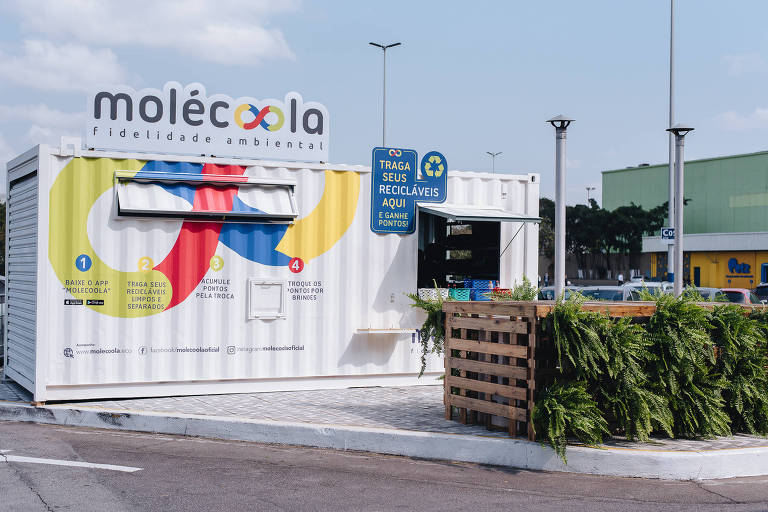
\includegraphics[width=0.7\linewidth]{produtos/prodquatro/molecoola}
	\caption{Contêiner do Molécoola}
	\label{fig:molecoola}
	\legend{Fonte: Jornal Folha de São Paulo}
\end{figure}
\FloatBarrier

\paragraph{\textbf{Armário Coletivo}}
Carina Zagonel é idealizadora do projeto “Armário Coletivo”, que consiste num “movimento de intervenção urbana que utiliza armários para transformar espaços públicos e criar novos hábitos de consumo. Eles são construídos a partir de materiais coletados nas ruas, produzidos com a ajuda da própria comunidade ”. O armário fica em um ponto escolhido estrategicamente no município ou no bairro em questão, os moradores podem ir até os armários e depositarem roupas, objetos que não utilizam mais. O outro morador que passa pelo local, pode abrir o armário e escolher o que ele deseja lá de dentro e ao tirar o item ele deve depositar algo em troca também. Em uma palestra da Carina Zagonel ela contou que num bairro rural de Florianópolis, os moradores acabavam deixando no armário frutas, verduras e legumes de seus pomares e hortas caseiros e essa ação gerou uma enorme troca (não só de roupas e objetos), mas também de variabilidade alimentar.

\begin{figure}[h]
	\centering
	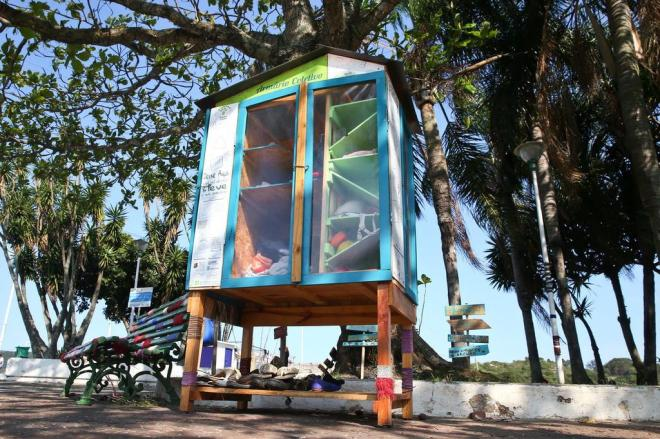
\includegraphics[width=0.7\linewidth]{produtos/prodquatro/armario_coletivo}
	\caption{Contêiner do Armário Coletivo}
	\label{fig:armario_coletivo}
	\legend{Fonte: Jornal Diário Catarinense}
\end{figure}


\newpage
\FloatBarrier
\section{Procedimentos operacionais e especificações mínimas a serem adotados nos serviços públicos de limpeza urbana e de manejo de resíduos sólidos}
\label{sec:proc_oper}
%% Manual item V
%% Entrega 1: 30.nov.2019
%% Autora: Maysa Rocha

De acordo com o item 1.2.1 Acondicionamento - Produto 3 - Diagnóstico do município de Monteiro Lobato/SP, o acondicionamento de resíduos comuns no município é composto por 59 lixeiras. Os resíduos comuns domiciliares e comerciais ficam normalmente armazenados em lixeira de ferro de dimensões (2x1x1 metros) ou lixeiras de madeira de dimensões (2x1x1 metros ou 1,20x1x1 metros). A problemática inserida é que apesar das lixeiras apresentarem um volume significativo, algumas classes de resíduos são dispostas inadequadamente no solo ao lado das lixeiras. Em vista disso, para erradicar o problema, é necessário um acondicionamento que possua uma porta de entrada, de modo que facilite tanto o trabalho do catador ou do agente de limpeza, quanto do morador que deposita o lixo no local adequado. O Departamento de Meio Ambiente de Flores da Cunha realizou a instalação de novas lixeiras para coleta seletiva no município (\autoref{fig:lixeirafloresdacunha}), que possuem as características descritas.   

\begin{figure}[h]
	\centering
	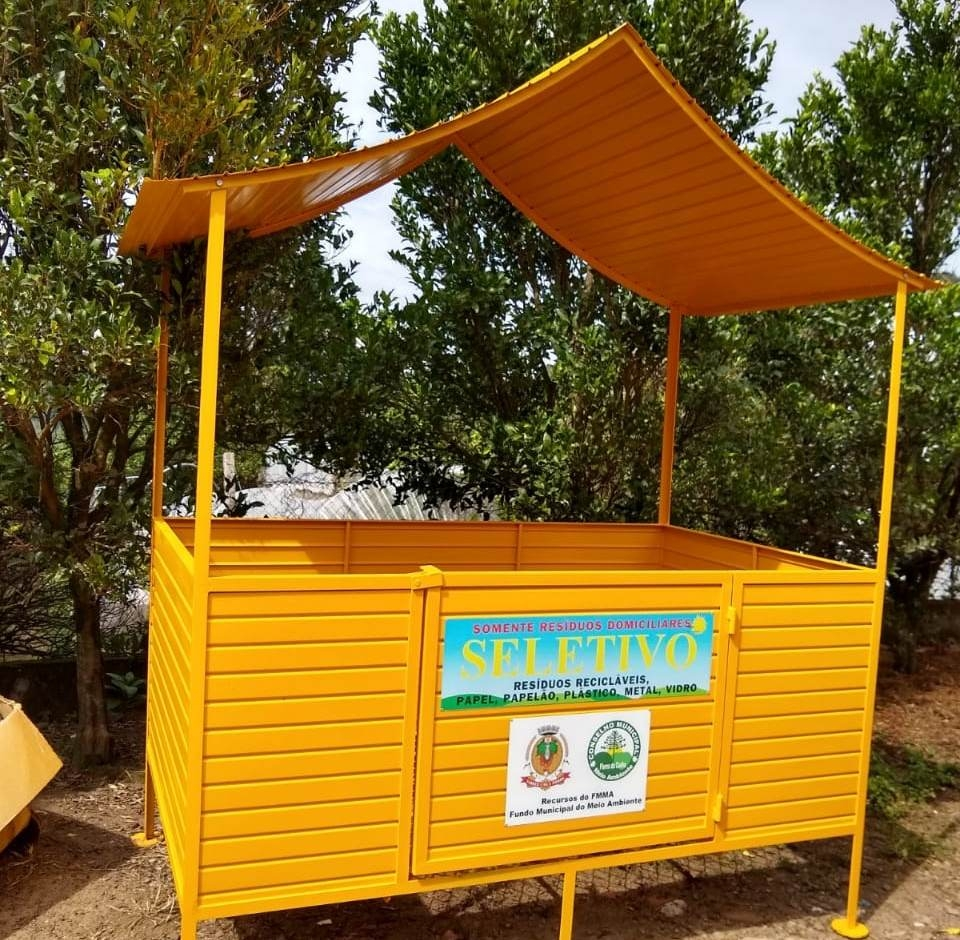
\includegraphics[width=0.5\linewidth]{produtos/prodquatro/lixeira_floresdacunha}
	\caption{Acondicionamento do município Flores da Cunha}
	\label{fig:lixeirafloresdacunha}
	\legend{Fonte: Jornal O Florense}
\end{figure}

Outras proposta interessante seria personalizar os acondicionamentos e fornecer dois para cada local ou criar uma divisória no mesmo, a fim de dividi-los entre resíduos orgânicos e recicláveis.
O Guia para elaboração dos Planos de Gestão de Resíduos Sólidos, disponibilizado pelo Ministério do Meio Ambiente discorre sobre um “Estudo de Regionalização”, que deve pré-dimensionar as instalações e sua localização adequada para a gestão dos resíduos sólidos em cada arranjo intermunicipal, tais como: pontos de entrega de resíduos, galpões de triagem dos resíduos secos, compostagem de resíduos orgânicos, instalações de tratamento dos resíduos dos serviços de saúde, aterros sanitários, aterros de resíduos da construção civil e inertes e outras instalações que permitam o manejo diferenciado e integrado dos diversos tipos de resíduos gerados na UF. Dentre as unidades e infraestruturas para a destinação final de resíduos podem ser citadas: 


\begin{itemize}
	\item LEV – Locais de Entrega Voluntária para Resíduos Recicláveis. Dispositivos de recebimento de recicláveis, como contêineres ou outros; 
	\item PEV – Pontos de Entrega Voluntária para RCC e Resíduos Volumosos, para acumulação temporária de resíduos da coleta seletiva e resíduos com logística reversa (conforme NBR 15.112/2004);
	\item Galpão de triagem de recicláveis secos; 
	Unidades de valorização de orgânicos (compostagem e biodigestão);
	\item ATT – Áreas de Triagem, Reciclagem e Transbordo de RCC, Volumosos e resíduos com logística reversa;
	\item Aterros sanitários (NBR 13.896/1997);
	\item ASPP - Aterro Sanitário de Pequeno Porte (NBR 15.849/2010); 
	\item Aterros de RCC Classe A (NBR 15.113/2004).
\end{itemize}

A Confederação Nacional de Municípios (CNM) destaca a diferença entre o Ponto de Entrega Voluntária (PEV), conhecidos também como Ecopontos, e o Local de Entrega Voluntária (LEV). PEV ou Ecoponto são locais, determinados pelas prefeituras, com equipamentos destinados para a acumulação temporária de resíduos da construção e demolição, de resíduos volumosos, da coleta seletiva e resíduos com logística reversa. Esses locais são amplos e com espaços bem definidos para cada tipo de resíduo a ser depositado no local. Os LEVs são locais de Entrega Voluntária de Resíduos Recicláveis, são contêineres, sacos ou outros dispositivos instalados em espaços públicos ou privados monitorados, para recebimento de recicláveis. A principal diferença entre eles é que os PEVs recebem resíduos volumosos e que fazem parte da logística reversa. Os LEVs são equipamentos menores, mas também aptos a armazenarem resíduos da coleta seletiva.

\newpage
\FloatBarrier
\section{Indicadores para os serviços públicos de limpeza urbana e de manejo de resíduos sólidos}
\label{sec:indicadores}
%% Manual item VI
%% Entrega 3: 26.nov.2019
%% Autora: Laís Shiki

No Produto 3 - Diagnóstico Municipal - deste \gls{pmgirs}, foram levantados os indicadores para os serviços públicos de limpeza urbana e de manejo de resíduos. Logo, neste Produto 4 não será discutido mais indicadores, visto que os tratados anteriormente já foram o suficiente na concepção deste plano.

\newpage
\FloatBarrier
\section{Regras para o transporte e outras etapas do gerenciamento de resíduos sólidos sujeitos ao plano de gerenciamento específico}
\label{sec:regras_trans}
%% Manual item VII
%% Entrega 1: 30.nov.2019
%% Autora: Lia Yukari

Para a elaboração dessa seção, foi considerado o disposto na \gls{pnrs} (Lei Federal nº 12.305/2010) e seu regulamento (Decreto nº 7.404/2010); tão bem como diversas outras normas dispostas e referenciadas de acordo com seu respectivo tipo de resíduo.

Aos resíduos sólidos como um todo, salienta-se normas a serem usadas como referência e importante para capacitação técnica e concordância de práticas relacionadas à resíduos:

\begin{itemize}
	\item \gls{nbr} 10004/04 – Resíduos sólidos – Classificação \cite{abnt:10004};
	\item \gls{nbr} 12980/93 - Coleta, varrição e acondicionamento de resíduos sólidos urbanos - Terminologia \cite{abnt:12980:1993};
	\item \gls{nbr} 7500/01 – Identificação para o transporte terrestre, manuseio, movimentação e armazenamento de produtos \cite{abnt:7500:2001}.
\end{itemize}

Para os resíduos que se classificam como resíduos perigosos (vide \cite{abnt:10004}), tem-se como base as normas:

\begin{itemize}
	\item \gls{nbr} 12235/92 – Armazenamento de resíduos perigosos \cite{abnt:12235:1992};
	\item \gls{nbr} 7501/11 – Transporte terrestre de produtos perigosos – terminologia \cite{abnt:7501:2011}; 
	\item \gls{nbr} 10157/87 – Aterros de resíduos perigosos – critérios para projetos, construção e operação \cite{abnt:10157:1987}.
\end{itemize}

Com base no Diagnóstico Municipal de Monteiro Lobato (Produto 3), evidenciou-se a proeminência de quatro tipos de resíduos gerados no município. Para tais, foram levantadas as devidas normas para seu transporte adequado, desde armazenamento a disposição final. São eles:

\begin{itemize}
	\item \gls{rsu}: comum e seletivo;
	\item \gls{rcc};
	\item \gls{rss};
	\item Resíduos de Logística Reversa.
\end{itemize}

	\subsection{Resíduos Sólidos Urbanos (RSU)}
	Os \gls{rsu} compreendem os resíduos domiciliares e os resíduos de limpeza urbana. Os resíduos domiciliares são os resíduos originários de atividades domésticas em residências urbanas. Os resíduos de limpeza urbana englobam os resíduos originários de varrição, de limpeza de logradouros, de vias públicas e de capina e poda \cite{brasil:12305, brasil:11445}.
	
	No município de Monteiro Lobato os \gls{rsu} são divididos em duas categorias: resíduos sólidos comuns e resíduos sólidos recicláveis. Os resíduos sólidos comuns no município consistem em resíduos considerados domiciliares (com exceção de recicláveis), rejeitos e matéria orgânica.
	
	Os resíduos oriundos de serviços de limpeza urbana como varrição, desobstrução de sarjetas, poda e capina são usualmente considerados pelo município como resíduos comuns e recebem, em sua maioria, a mesma destinação e disposição final que os resíduos domiciliares e de estabelecimentos comerciais e prestadores de serviços.
	
	Os resíduos sólidos recicláveis são constituídos de materiais plásticos de diversas categorias, vidro, metal, papel e papelão; que possuem valor agregado e devem voltar ao sistema produtivo como matéria prima para fabricação de novos produtos através da reciclagem e/ou reaproveitamento.
	
	Atualmente, o município de Monteiro Lobato possui apenas um tipo de lixeira para o armazenamento pré-coleta, a lixeira não possui separação física para os resíduos comuns e recicláveis, podendo assim causar uma contaminação inicial caso ambos tipos de resíduos estejam dispostos concomitantemente. O município irá proporcionar novos tipos de lixeiras, e possíveis modelos encontram-se na \autoref{sec:proc_oper}.
	
	A coleta dos resíduos deve estar de acordo com as características dispostas na \gls{nbr} 13463 \cite{abnt:13463:1995}. Além de que, após diagnóstico realizado no município de Monteiro Lobato, é importante que haja uma política de capacitação técnica com os funcionários responsáveis pela coleta, tão bem como a disponibilizaçao de \gls{epi}. 
	
	A capacitação técnica dos funcionários também é importante quando refere-se ao transporte terrestre dos resíduos, tem-se como embasamento a \gls{nbr} 13221/03. O transporte deve ser feito por meio de equipamento adequado, obedecendo às regulamentações pertinentes \cite{abnt:13221:2003}. Atualmente, no município de Monteiro Lobato, é realizado apenas a manutenção corretiva da frota, a qual pode acarretar em uma possível paralisação temporária da coleta e transporte dos resíduos comum e reciclável. É fundamental que ocorra, com uma certa frequência, a manutenção e revisão dos meios de transporte dos resíduos, de modo preventivo; a fim de se garantir a funcionalidade dos equipamentos utilizados no gerenciamento dos resíduos sólidos.
	
	O estado de conservação do equipamento de transporte deve ser tal que, durante o transporte, não permita vazamento ou derramamento do resíduo. O resíduo, durante o transporte, deve estar protegido de intempéries,  assim como deve estar devidamente
	acondicionado para evitar o seu espalhamento na via pública ou via férrea. A descontaminação dos equipamentos de transporte deve ser de responsabilidade do gerador e deve ser realizada em local(is) e sistema(s) previamente autorizados pelo órgão de controle ambiental competente \cite{abnt:13221:2003}.
	
	O transporte sem vazamento ou derramamento deve ser garantido desde o momento de coleta até o seu local de disposição final, sendo essa disposição sem danos à saúde pública e à  segurança, tendo os seus impactos ambientais minimizados \cite{abnt:8419}. É de extrema importância listar possíveis locais para disposição final dos resíduos comuns e recicláveis, caso seja necessário o estabelecimento de uma ação emergencial, como encontra-se descrito na \autoref{sec:emerg_corr}.
	
	\subsection{Resíduos de Construção Civil (RCC)}
	\label{subsec:trans_rcc}
	\gls{rcc} são aqueles gerados das atividades de construções, reformas, reparos e demolições de obras de construção civil, incluindo os resíduos derivados da preparação e escavação de terrenos para obras civis, tais como: tijolos, blocos cerâmicos, concreto em geral, solos, rochas, metais, resinas, colas, tintas, madeiras e compensados, forros, argamassa, gesso, telhas, pavimento asfáltico, vidros, plásticos, tubulações, fiação elétrica, entre outros. Os \gls{rcc} são comumente denominados de entulhos de obras, caliça ou metralha \cite{brasil:12305, conama:307}. 
	
	A \gls{ssm} de Monteiro Lobato é responsável pela coleta dos \gls{rcc}. O serviço prestado pela prefeitura é taxado do solicitante através da cobrança de R\$ 41,82 por hora de serviço e por R\$ 25,09 por hora do uso do caminhão basculante. A quantidade e frequência em que ocorrem as coletas não são catalogadas internamente, dificultando assim, sua posterior análise e possíveis ações de melhoria para o manejo desse tipo de resíduo.
		
	Os \gls{rcc} gerados são armazenados na calçada em frente ao imóvel da respectiva construção civil até que seja realizada a coleta pela \gls{ssm}. Após a coleta, os \gls{rcc} são armazenados ao ar livre no pátio da prefeitura no bairro Morada do Sol,  onde observa-se a disposição inadequada dos resíduos em solo exposto e ao ar livre. Os \gls{rcc} são utilizados em estradas vicinais e nas valetas e buracos com erosões, quando necessário.
	
	Desse modo, recomenda-se o registro de cada uma das coletas, com sua respectiva data, horário, quantidade de \gls{rcc}, nome do solicitante, valor da taxa e qualquer outro tipo de informação que seja válida.
	
	Quanto ao armazenamento do \gls{rcc}, é importante a presença de uma área de transbordo adequada (bota fora regularizado); em que o resíduo não esteja exposto à chuva, sol intenso, vetores e animais. Faz-se também importante que o resíduo não esteja em contato direto com o solo, a fim de se evitar contaminações no mesmo ou em águas pluviais; para tal, recomenda-se o uso de recepientes adequados ou uma camada impermeabilizada.
	
	Ademais, o resíduo é reaproveitado no município conforme demanda dos próprios munícipes. É possível elaborar projetos de reaproveitamento dos \gls{rcc} em construções civis e também para manutenção das estradas - como é realizado atualmente; mas de modo controlado, analisado, seguro e estável.
	
	\subsection{Resíduos do Sistema de Saúde (RSS)}
	Os \gls{rss} são definidos como os resíduos provenientes de atividades de atendimento à saúde humana ou animal, incluindo os serviços de assistência domiciliar e de trabalhos de campo; laboratórios analíticos de produtos para saúde; necrotérios, funerárias e serviços onde se realizem atividades de embalsamamento; serviços de medicina legal; drogarias e farmácias inclusive as de manipulação; estabelecimentos de ensino e pesquisa na área de saúde; centros de controle de zoonoses; distribuidores de produtos farmacêuticos; importadores, distribuidores e produtores de materiais e controles para diagnóstico in vitro; unidades móveis de atendimento à saúde; serviços de acupuntura; serviços de tatuagem, entre outros similares \cite{conama:362}.
	
	No município de Monteiro Lobato há a presença de uma \gls{ubs} (realiza serviço 24 horas de pronto atendimento e atendimento de ambulatório de segunda-feira à sexta-feira) e mais sete principais estabelecimentos geradores de \gls{rss} (que englobam veterinários, consultórios odontológicos, farmácia e estabelecimento de comércio de produtos para animais). 
		
	Tanto a \gls{ubs} quanto a maioria dos estabelecimentos geradores de \gls{rss} não dispõem de um \gls{pgrss}. Com base no diagnóstico elaborado, algumas defasagens relacionadas ao tratamento dos resíduos nos estabelecimentos de saúde foram identificados, tais como a segregação incorreta dos resíduos comuns e recicláveis, a forma adequada de acondicionamento do \gls{rss} de acordo com sua respectiva classe e o local de armazenamento temporário.
	
	A maioria dos estabelecimentos geradores de \gls{rss} encaminham seus resíduos à \gls{ubs} do município, a qual os armazena em um ambiente específico. A  empresa especializada AGIT Soluções Ambientais Ltda é a responsável pelo serviço de coleta (de 15 em 15 dias), transporte e incineração que ocorre no município de Itajubá. 
	
	Desse modo, é importante a presença de um \gls{pgrss}, prioritariamente a \gls{ubs} do município por acondiocionar o \gls{rss} de outros estabelecimentos. Para um correto tratamento do \gls{rss}, foi utilizado como referência o Manual da \gls{anvisa}, de 2006, apresentado no Produto 3 (diagnóstico).
	
	Ademais, acentua-se duas normas importantes ao tratar-se da capacitação técnica de funcionários dentro de um estabelecimento de saúde, definindo a terminologia em relação aos \gls{rss} e os procedimentos exigíveis para garantir condições de higiene e segurança no processamento interno de resíduos infectantes, especiais e comuns, nos serviços de saúde. São elas, respectivamente \cite{abnt:12807:1993, abnt:12809:1993}:
	
	\begin{itemize}
		\item \gls{nbr} 12807/93 – Resíduos de serviços de saúde
		\item \gls{nbr} 12809/93 – Manuseio de resíduos de saúde
	\end{itemize}
	
	Por fim, em 2018, a \gls{anvisa} - através de uma \gls{rdc} - regulamentou os requisitos de Boas Práticas de Gerenciamento dos \gls{rss}. Em seu Art. 5º, estabelece que todo serviço gerador deve dispor de um \gls{pgrss}, observando as regulamentações federais, estaduais, municipais ou do Distrito Federal \cite{anvisa:222:2018}.

	
	Em seu Art. 6º, estabelece condições mínimas ao gerador de \gls{rss}, as quais devem estar coincidentes ao \gls{pgrss}. Alguns exemplos são \cite{anvisa:222:2018}:
	
	\begin{itemize}
		\item descrever os procedimentos relacionados ao gerenciamento dos \gls{rss} quanto à geração, à segregação, ao acondicionamento, à identificação, à coleta, ao armazenamento, ao transporte, ao tratamento e à disposição final ambientalmente adequada;
		\item  estar em conformidade com a regulamentação sanitária e ambiental, bem como com as normas de coleta e transporte dos serviços locais de limpeza urbana;

		\item estar em conformidade com as rotinas e processos de higienização e limpeza	vigentes no serviço gerador de \gls{rss};
		\item descrever os programas de capacitação desenvolvidos e implantados pelo serviço gerador abrangendo todas as unidades geradoras de \gls{rss} e o setor de limpeza e conservação.
	\end{itemize}
	
	\subsection{Resíduos de Logística Reversa}
	Uma das ferramentas propostas na \gls{pnrs}, para auxiliar na busca por atingir a logística reversa, é a responsabilidade compartilhada pelo ciclo de vida dos produtos. Os fabricantes, os importadores, os distribuidores e os comerciantes têm responsabilidade no recolhimento dos produtos e dos resíduos remanescentes após o uso, assim como sua subsequente destinação final ambientalmente adequada destes resíduos \cite{brasil:12305}.
	
	No diagnóstico de resíduos sólidos realizado no município de Monteiro Lobato, foi levantada uma lista dos estabelecimentos geradores de resíduos provenientes de logística reversa. Assim, com base na responsabilidade compartilhada supracitada, cabe ao munícipio o acompanhamento e fiscalização das unidades para certificar-se que estão sendo realizadas as devidas destinações finais adequadas. 
	
	O acompanhamento pode ser realizado através da disponibilização de um funcionário, ao menos uma vez por semestre, para visita e monitoramento nos estabelecimentos listados; de modo que ocorra o controle e fiscalização dos mesmos em relação à logística reversa.
	
\newpage
\section{Definição de Responsabilidades} %quanto à implementação e operacionalização do Plano
\label{sec:def_resp}
%% Manual item VIII
%% Entrega 1: 30.nov.2019
%% Autora: Talita Guerra
	
A \gls{pnrs} estabelece o conceito de responsabilidade compartilhada pelo ciclo de vida dos produtos para a gestão e gerenciamento dos resíduos gerados nos territórios. Por responsabilidade compartilhada entende-se o "conjunto de atribuições individualizadas e encadeadas dos fabricantes, importadores, distribuidores e comerciantes, dos consumidores e dos titulares dos serviços públicos de limpeza urbana e de manejo dos resíduos sólidos, para minimizar o volume de resíduos sólidos e rejeitos gerados, bem como para reduzir os impactos causados à saúde humana e à qualidade ambiental decorrentes do ciclo de vida dos produtos" \cite{brasil:12305}.

Ao poder público municipal cabe a responsabilidade de implementação deste plano e articular com os setores da sociedade para o cumprimentos de ações e metas para e melhoria da gestão e gerenciamento dos resíduos contidas neste plano e que possam surgir no decorrer de sua implementação e duração.

Ao setor privado cabe a elaboração e aplicação de \gls{pgrs} específicos, quando determinado for, que deve conter os requisito mínimos deste tipo de plano. 

À sociedade cabe observar e implantar as medidas privadas e comunitárias cabíveis que ajudarão no cumprimento das metas estabelecidas neste plano e das metas que possam surgir no decorrer da vigência deste plano. 

%	A definição das responsabilidades deve ser feita quanto à implementação e à operacionalização do Plano, incluídas as etapas dos planos de gerenciamento de resíduos a que se refere o art. 20 da Lei Federal nº 12.305/2010 a cargo do poder público. 

%	Conforme o conceito de responsabilidade compartilhada pelo ciclo de vida do produto, devem ser definidas as atribuições individualizadas e encadeadas dos fabricantes, importadores, distribuidores e comerciantes, dos consumidores e dos titulares dos serviços públicos de limpeza urbana e manejo de resíduos sólidos. 
	
\FloatBarrier
\newpage
\section{Programas e ações de capacitação técnica voltados para implementação e operacionalização do Plano}
\label{sec:capac_tec}
%% Manual item IX
%% Entrega 1: 30.nov.2019
%% Autora: Lia Yukari

Essa seção discorre sobre possibilidades de capacitação técnica àqueles envolvidos na implementação e operacionalização desse \gls{pmgirs}. No diagnóstico, pôde-se avaliar deficiências relacionadas à assistência técnica e à clareza e propagação dos conhecimentos relacionados a resíduos sólidos. Com base nisso, podem ser definidos programas e ações a serem adotados em prol de uma melhor funcionalidade desse instrumento legal.

A \autoref{tab:capacit_tec} apresenta os Programas e Ações recomendados ao município de Monteiro Lobato, referente a sua capacitação técnica, seu respectivo público-alvo, modo e frequência de implementação.

	% Table generated by Excel2LaTeX from sheet 'capacit_tec'
\begin{table}[htbp]
	\centering
	\caption{Programas e Ações de Capacitação Técnica para o Município de Monteiro Lobato}
	\resizebox{\textwidth}{!}{%
	\begin{tabular}{p{12.955em}p{12.955em}p{20.59em}}
		\rowcolor[rgb]{ .969,  .588,  .275} \textcolor[rgb]{ 1,  1,  1}{\textbf{Programas e Ações}} & \textcolor[rgb]{ 1,  1,  1}{\textbf{Público-Alvo}} & \textcolor[rgb]{ 1,  1,  1}{\textbf{Implementação}} \\
		\rowcolor[rgb]{ .992,  .914,  .851} Envolvimento do Poder Executivo Municipal com as ações estabelecidas no PMGIRS & Prefeitura e secretarias municipais que encontram-se envolvidas, direta ou indiretamente, na área de resíduos sólidos & Realização de reuniões bimestrais com todos os envolvidos (ou ao menos um representante), para definição de como as ações detalhadas no PMGIRS serão implementadas \\
		\rowcolor[rgb]{ .984,  .831,  .706} Envolvimento dos funcionários municipais com as ações estabelecidas no PMGIRS & Todos os funcionários municipais que trabalham, direta ou indiretamente, na área de resíduos sólidos & Realização de reuniões semestrais com todos os funcionários municipais e Poder Executivo, para deliberação de como as ações detalhadas no PMGIRS serão implementadas \\
		\rowcolor[rgb]{ .992,  .914,  .851} Apoio técnico de especialistas, de escolas ou universidades e de instituições voltadas à área de resíduos sólidos & Poder Executivo Municipal, funcionários e munícipes de Monteiro Lobato & Estabelecimento de parcerias com escolas, universidades ou instituições para estudo da implementação e acompanhamento trimestral da operacionalização das ações detalhadas no PMGIRS.  \\
		\rowcolor[rgb]{ .984,  .831,  .706} Envolvimento da população com as ações estabelecidas no PMGIRS & Munícipes de Monteiro Lobato & Ampla divulgação das audiências do PMGIRS. Propagação contínua do conteúdo do PMGIRS; através de informativos, mídias sociais e disseminação em eventos, instituições e escolas. \\
		\rowcolor[rgb]{ .992,  .914,  .851} Apresentação de dados na base SNIS & Prefeitura e secretarias municipais que encontram-se envolvidas, direta ou indiretamente, na área de saneamento básico & Abastecimento mensal de dados e informações do município, para controle e futura análise das ações implementadas no PMGIRS. \\
	\end{tabular}%
}
	\label{tab:capacit_tec}%
\end{table}%

	
É importante salientar que a responsabilidade de implementação e operacionalização é inteiramente do município, o qual cabe ao mesmo firmar qualquer tipo de apoio técnico que seja necessário ou conveniente. Assim, como auxílio de capacitação técnica, entende-se a disponibilidade para consultoria relacionada ao gerenciamento dos resíduos sólidos e a orientação das ações prescritas nesse Produto.

As linhas de ações principais são aquelas voltadas à educação ambiental e as preventivas e corretivas; tão bem como o cumprimento das metas de redução, reutilização, coleta seletiva e reciclagem, entre outras, com vistas a reduzir a quantidade de rejeitos encaminhados para disposição final ambientalmente adequada.

\FloatBarrier
\newpage
\section{Programas e ações de educação ambiental}
\label{sec:educ_amb}
%% Manual item X
%% Entrega 3: 26.nov.2019
%% Autora: Talita Guerra e Maysa Rocha

\label{sec:educ_amb}
O termo "educação ambiental" possui diversas definições. Uma delas foi descrita no Congresso de Belgrado, promovido pela UNESCO em 1975, e foi compreendida como um processo que visa: “(...) formar uma população mundial consciente e preocupada com o ambiente e com os problemas que lhe dizem respeito, uma população que tenha os conhecimentos, as competências, o estado de espírito, as motivações e o sentido de participação e engajamento que lhe permita trabalhar individualmente e coletivamente para resolver os problemas atuais e impedir que se repitam (...)" 

O \gls{mma} retrata a ideia central da \gls{pnrs} como uma transformação da visão sobre os resíduos sólidos, o que antes era visto como uma reta (desde a extração da matéria prima até o "jogar o lixo fora"), agora é visto como um ciclo onde as pontas se juntam (o que antes era lixo, inútil, torna-se recurso em potencial). Esse princípio de gestão integrada de resíduos busca incorporar e denominar como responsável quem legisla, quem produz, quem consome, quem recicla e quem cuida do destino final. Em outras palavras, estabelece a responsabilidade compartilhada por todos os entes da sociedade pela geração e manejo dos resíduos sólidos. 

Essa mudança de visão sobre os resíduos muitas vezes não é imediata ou natural; o habitual é usar e descartar, afastar o que não serve mais da vista. Logo, há a necessidade de investir-se em políticas voltadas à educação ambiental com foco na transformação do pensar sobre o que é "lixo", buscando um novo olhar para os hábitos costumeiros de consumo e descarte, incentivando a criatividade como propulsora de ideias e ações para a resolução de questões relacionadas aos resíduos.

\subsection{Objetivos}

Os programas e ações de educação ambiental tem como objetivo principal incentivar à participação comunitária ativa, de modo que consigam compreender de forma integrada o meio ambiente e suas relações cotidianas, que envolvem aspectos: psicológicos, históricos, políticos, sociais, econômicos, culturais, tecnológicos e éticos. Compreender essa questão integrada torna a educação ambiental uma ferramenta de grande importância para implementar pequenas mudanças que trarão benefícios pessoais e ambientais,  pois irão influenciar nas atividades locais, por exemplo: qualidade de vida, escolhas de consumo, cultura da descartabilidade, limpeza do município, erradicação dos vetores de doenças, entre outros pontos. 

\subsection{Público-alvo}

É importante enfatizar que a educação ambiental não se restringe apenas ao âmbito escolar. Muito além que trabalha-la com crianças e jovens regularmente matriculados em instituições de ensino, a educação ambiental necessita abranger a comunidade como um todo: as crianças, seus pais e professores; as empresas e os funcionários; as comunidades de moradores; os turistas; o poder público. Logo, o público-alvo das ações voltadas à Educação Ambiental compreende toda a comunidade Lobatense.

\subsection{Metas, projetos e ações}

As ações em educação ambiental para a questão dos resíduos sólidos devem e promover, na seguinte ordem os princípios da:
\begin{itemize}
	\item não geração de resíduos;
	\item redução de resíduos;
	\item reutilização de resíduos;
	\item reciclagem de resíduos;
\end{itemize} 

O diálogo e a articulação entre os entes das sociedade Lobatense devem ser estimulados pelo poder público, para identificação de soluções individuais ou coletivas que por ventura já sejam realizadas e que possam ser replicadas ou adaptadas em outras comunidades e setores da sociedade. A comunicação horizontal entre os setores da sociedade pode aflorar nos cidadãos o sentimento de responsabilidade pelos cuidados com a questão dos resíduos sólidos e proporcionar meios para que mudanças positivas aconteçam no território.

\subsubsection{Priorização da educação ambiental nos currículos escolares}
De acordo com (LIMA, 2004) um dos maiores campos de atuação da \gls{ea} é a escola, um espaço privilegiado, onde se pode criar condições e alternativas que estimulem os alunos a terem concepções e posturas cidadãs, cientes de suas responsabilidades e principalmente, integrantes do meio ambiente. Nessa perspectiva, a escola pode constituir um espaço para o desenvolvimento da EA objetivando formar cidadãos conscientes, capazes de enfrentar os desafios da realidade socioambiental.

Sabe-se que a educação ambiental não se restringe apenas ao âmbito escolar e que necessita abranger a comunidade como um todo. Entretanto é de suma importância que as escolas municipais e particulares abordem essa temática integrando-a às matérias da grade curricular. Incentivar e ensinar as crianças e adolescentes, desde novos, os hábitos corretos na segregação dos resíduos, na economia de energia e água, na destinação correta do "lixo doméstico", no potencial de reciclagem, no consumo consciente, na cultura da descartabilidade, nos problemas acarretados pela falta da educação ambiental em si, entre outros, perpetuam uma sociedade futura com indivíduos mais conscientes e interessados.

Portanto, uma das metas a serem realizadas pelo município de Monteiro Lobato, é incluir a educação ambiental no currículo escolar de todas as escolas municipais da região. A proposta é que essa meta seja realizada em curto prazo (aproximadamente 4 anos).

\subsubsection{Segregação dos resíduos}
Segundo o \gls{mma}, segregar o resíduo de maneira correta reúne diversas vantagens tanto para o meio ambiente quanto para a sociedade, pois além da correta separação do lixo doméstico aliviar lixões e aterros sanitários, chegando até eles apenas os rejeitos (restos de resíduos que não podem ser reaproveitáveis), grande parte dos resíduos sólidos gerados em casa pode ser reutilizada. A reciclagem economiza recursos naturais e gera renda para os catadores de lixo, parte da população que depende dos resíduos sólidos descartados para sobreviver.

Além da importância da segregação correta do resíduo, é importante também certificar o encaminhamento e destino correto do mesmo. De acordo com o produto 3, quase 25 \% do resíduo gerado pela população é reciclável mas tem como destino final o aterro sanitário.
Portanto segregar o resíduo doméstico de uma forma correta é uma meta para o município de Monteiro Lobato, que deve ser cumprida a curto prazo (aproximadamente 4 anos). A sociedade e o poder público pode incentivar e disseminar o assunto através de oficinas e projetos com lideranças locais.

%\subsubsection{Projetos e ações - Segregação dos resíduos}
A proposta para incentivar e disseminar a segregação correta dos resíduos consiste em, primeiramente, alcançar todos os munícipes da região com informações corretas sobre a separação, pois a segregação de forma errada pode acontecer por falta de conhecimento. Esse alcance pode ser disseminado através de oficinas, cartilhas, conteúdo em redes sociais, reuniões grupais, dinâmicas, entre outros. O \gls{mma} explica como separar o "lixo" corretamente e essas informações podem fazer parte dos eventos citados anteriormente:
\begin{itemize}
	\item Não misturar recicláveis com orgânicos - sobras de alimentos, cascas de frutas e legumes. 
	\item Colocar plásticos, vidros, metais e papéis em sacos separados.
	\item Lavar as embalagens do tipo longa vida, latas, garrafas e frascos de vidro e plástico. Secá-los antes de depositar nos coletores. (É importante enfatizar que provavelmente os recicláveis serão transportados para um local de triagem ou manuseado por outras pessoas e armazenados em um local até serem enviados para o local apropriado de fato, com isso a lavagem das embalagens é de grande apreço pois não gerará mau cheiro para outras pessoas que vão tratar daquele resíduo )
	\item Papéis devem estar secos. Podem ser dobrados, mas não amassados.
	\item Embrulhar vidros quebrados e outros materiais cortantes em papel grosso (do tipo jornal) ou colocá-los em uma caixa para evitar acidentes. Garrafas e frascos não devem ser misturados com os vidros planos.	
\end{itemize} 
Os rejeitos, aqueles que vão direto para o aterro sanitário pois não possuem condições de serem reciclados e condições de algum tratamento pós uso, são: 
\begin{itemize}
	\item Papel-carbono, etiqueta adesiva, fita crepe, guardanapos, fotografias, filtro de cigarros, papéis sujos, papéis sanitários, copos de papel. Cabos de panela e tomadas. Clipes, grampos, esponjas de aço, canos. Espelhos, cristais, cerâmicas, porcelana. 
\end{itemize}

O óleo de cozinha usado também é um resíduo que deve ser corretamente segregado por também ter potencial de contaminação. O município de Monteiro Lobato já possui coleta de óleo de cozinha em um ponto da cidade mas que não abrange todos os munícipes. A proposta para melhorar a segregação desse item é expandir os pontos de coleta de óleo para pelo menos 2 na região central e ao menos um ponto em cada bairro, posicionados em vias de passagem que se mostrem estratégicas. Pontos de coleta em escolas e em centros comunitários são incentivados, juntamente com ideias e ações para o reaproveitamento do material dentro das comunidades.   

Outra proposta para incentivar a correta segregação dos resíduos é a instalação de composteiras de resíduos orgânicos nos prédios públicos, além da instalação de recipientes para o armazenamento de materiais recicláveis secos e limpos gerados no próprio local (papéis, embalagens, copos descartáveis ocasionais), desestimulando a mistura desses resíduos. É importante que os espaços administrados pela Prefeitura sejam locais de exemplo de educação ambiental para os munícipes. A implantação dessas medidas deverá ocorrer em curto período (até dois anos).  


\FloatBarrier
\newpage
\section{Mecanismos para a criação de fontes de negócios, emprego e renda}
\label{sec:mec_renda}
%% Manual item XII
%% Entrega 3: 26.nov.2019
%% Autora: Laís Shiki

Para a adequada gestão dos resíduos sólidos é necessário, primeiramente, a compreensão da importância que estes materiais podem ainda possuir. Assim, vale ressaltar que "o resíduo sólido reutilizável e reciclável deve ser reconhecido como um bem econômico e de valor social, gerador de trabalho e renda, além de promover a cidadania e o incentivo à criação e desenvolvimento de cooperativas e outras formas de associação de catadores de materiais reutilizáveis e recicláveis e à indústria da reciclagem [...]" \cite{agevap_manual_2019}. Tendo em vista a função de gerar trabalho e renda, este \gls{pmgirs} propõe algumas sugestões a serem implementadas no município.

\subsection{Criação de uma cooperativa ou outra forma de associação de catadores de materiais reutilizáveis e recicláveis}

Um dos objetivos da \gls{pnrs} é a integração dos catadores de materiais reutilizáveis e recicláveis. Em Monteiro Lobato há alguns coletores informais, que foram constatados durante as visitas técnicas. A princípio, o poder público local poderia se reunir com estes a fim de compreender a realidade de trabalho, atentando-se especialmente com as dificuldades e deficiências encontradas por estes. Durante a reunião pode ser questionado o interesse destes catadores em formalizar seu trabalho, através da criação de uma cooperativa ou outra forma de associação, sendo levantadas as etapas do processo e os benefícios.

Existem projetos relevantes ao assunto que podem ser estudados pelo município. Um deles é o Programa Pró-Catador (Decreto n° 7.405/2010), cuja finalidade é "integrar e articular as ações do Governo Federal voltadas ao apoio e ao fomento à organização produtiva dos catadores de materiais reutilizáveis e recicláveis, à melhoria das condições de trabalho, à ampliação das oportunidades de inclusão social e econômica e à expansão da coleta seletiva de resíduos sólidos, da reutilização e da reciclagem por meio da atuação desse segmento" \cite{brasil:7405}.

É importante para a escolha de qual forma de sistema, seja associação ou seja cooperativa, que será estabelecido no município, compreender as diferenças entre ambas. Para tanto, a \autoref{tab:cooper_associa} apresenta as principais características de cada.

% Table generated by Excel2LaTeX from sheet 'cooper_associa'
\begin{table}[htbp]
  \centering
  \arrayrulecolor{white}
  \caption{Diferenças entre cooperativas e associações.}
  %\resizebox{\textwidth}{!}{
    \begin{tabular}{P{17.955em}|P{17.955em}}
    \rowcolor[rgb]{ .969,  .588,  .275} Cooperativa & Associação \\
    \rowcolor[rgb]{ .992,  .914,  .851} Os participantes são os donos do patrimônio e os beneficiários dos ganhos & Os associados não são propriamente os donos \\
    \rowcolor[rgb]{ .984,  .831,  .706} Beneficia os próprios cooperados & O patrimônio acumulado, no caso de sua dissolução, deve ser destinado a outra instituição semelhante, conforme determina a lei \\
    \rowcolor[rgb]{ .992,  .914,  .851} Por meio de assembleia geral, as sobras das relações comerciais, podem ser distribuídas entre os cooperados & Os ganhos devem ser destinados à sociedade, e não aos associados \\
    \rowcolor[rgb]{ .984,  .831,  .706} Existe o repasse dos valores relacionados ao trabalho prestado pelos cooperados ou da venda dos produtos entregues na cooperativa & Na maioria das vezes, os associados não são nem mesmo os beneficiários da ação do trabalho da associação \\
    \rowcolor[rgb]{ .992,  .914,  .851} Mínimo de 20 pessoas & Mínimo de 2 pessoas \\
    \rowcolor[rgb]{ .984,  .831,  .706} Tem capital social (formado por quotas, podendo receber doações, empréstimos e processos de capitalização), o que facilita financiamentos em instituições financeiras  & Patrimônio formado por taxas pagas pelos associados, doações,  fundos e reservas. Não possui capital social \\
    \rowcolor[rgb]{ .992,  .914,  .851} Lei n° 5.764/1971; Constituição - art. 5°, de XVII a XXI, e art. 174, §2° e Código civil (Lei n° 10.406/2002)  & Constituição - art. 5°, de XVII a XXI, e art. 174, §2° e Código civil (Lei n° 10.406/2002)  \\
    \end{tabular}%
%}
  \label{tab:cooper_associa}%
  \legend{Fonte: \cite{cooper_associa}.}
\end{table}%


\FloatBarrier

Após a reunião, seria interessante a Prefeitura estudar maneiras de tornar viável a criação desse sistema. Por exemplo, ceder um terreno/espaço público para a construção de um galpão, tornando, assim, o espaço de trabalho destes catadores e auxiliar na compra de balanças, prensas, carrinhos e quaisquer outros equipamentos necessários para a operacionalização. Segundo o art. 42 da Lei Federal n° 12.305/2010, o Poder Público poderá instituir medidas indutoras e linhas de financiamento para atender a iniciativa de implantação de infraestrutura física e aquisição de equipamentos para cooperativas ou outras formas de associação de catadores \cite{brasil:12305}.

O art. 81 do Decreto n° 7.404/2010, cita que as instituições financeiras federais podem criar linhas especiais de financiamento para:

\begin{itemize}
	\item Cooperativas ou outras formas de associação de catadores de materiais reutilizáveis e recicláveis, com o objetivo de aquisição de máquinas e equipamentos utilizados na gestão de resíduos sólidos;
	\item Atividades destinadas à reciclagem e ao reaproveitamento de resíduos sólidos, bem como atividades de inovação e desenvolvimento relativas ao gerenciamento de resíduos sólidos; e 
	\item Atendimento a projetos de investimentos em gerenciamento de resíduos sólidos.
\end{itemize}

Em relação a documentação legal, no caso de se optar pelo sistema de cooperativa, é preciso que os cooperados elaborem, com o auxílio de um advogado, um estatuto que contenha todas as normas de administração que vão reger a cooperativa, tal documento deve ser aprovado em assembleia geral e registrado em Cartório. Posteriormente, deve-se obter CNPJ no Ministério da Fazenda/Receita Federal e realizar a inscrição no \gls{inss}. Além disso, é necessário obter na Prefeitura a inscrição municipal e concessão de alvará de licença de funcionamento. \cite{cooper_sebrae}. 

Atualmente, no município não há manutenção preventiva da frota de caminhões que realizam a coleta comum e seletiva. Apenas é feita a manutenção corretiva, que segundo a Prefeitura Municipal de Monteiro Lobato é efetuada com frequência, o que possivelmente indica a sobrecarga dos veículos. Assim, com a criação de uma cooperativa ou outra forma de associação, realizar um acordo para que em um dos dias da semana a coleta fosse realizada por estes trabalhadores, de modo que os caminhões passem por manutenção preventiva, será vantajoso para todas as partes envolvidas.   

\subsection{Ações para geração de fontes de negócios, trabalho e renda}

Conforme abordado na \autoref{sec:sol_cons}, Monteiro Lobato pode buscar soluções consorciadas ou compartilhadas com outros municípios visando a geração de fontes de negócios, trabalho e renda. Ademais, investigar meios para atrair pequenas empresas que atuam na área de beneficiamento de materiais recicláveis e/ou praticam a reciclagem em si, a se estabelecer no município seria de grande benefício. Medidas indutoras como incentivos fiscais, financeiros e creditícios e cessão de terrenos públicos, podem fomentar tal iniciativa \cite{agevap_manual_2019}. 

Outra ação que o poder público local pode exercer é, por exemplo, organizar grupos formados por interessados em desenvolver atividades artesanais a partir da reutilização e reciclagem de certos resíduos, como \cite{pmgirs_lagoinha_2017}:

\begin{itemize}
	\item Fabricação de sabão reaproveitando óleo de cozinha e gorduras, no município já há um ponto de entrega desse tipo de material localizado ao lado do Terminal rodoviário;
	\item Utilizar madeiras descartadas ou doadas para restaurar móveis antigos ou fabricar novos;
	\item Fabricação de produtos a partir de garrafas PET, como vassouras e artigos para decoração, já existem várias experiências neste sentido com o objetivo de elevação de renda para populações vulneráveis;
	\item Produzir itens com retalhos de tecidos, técnica conhecida como patchwork, por exemplo sacolas retornáveis, colchas, capas para almofadas e tapetes. Como foi visto no Produto 3 deste \gls{pmgirs}, em Monteiro Lobato há uma grande quantia de tecidos sendo descartados que poderiam ser reaproveitados para este fim.
\end{itemize}    

\FloatBarrier
\newpage
\section{Programas e ações para a participação de grupos interessados}
\label{sec:grup_int}
%% Manual item XI
%% Entrega 3: 26.nov.2019
%% Autora: Laís Shiki

É de extrema importância desenvolver certas estratégias para envolver grupos interessados de alguma forma na gestão dos resíduos sólidos do município, especialmente os catadores de materiais reutilizáveis e recicláveis, como foi discutido anteriormente, Monteiro Lobato não possui uma cooperativa ou outra forma de associação destes trabalhadores. Logo, na \autoref{sec:mec_renda} foram apresentados os principais passos para a criação desta sociedade, que é um dos objetivos da \gls{pnrs}.

Outro exemplo de grupo interessado é a de empresas recicladoras, seria interessante o município buscar formas para atrair estas que já atuam em um município vizinho ou até mesmo buscar soluções consorciadas que envolvem elas. Outra opção seria a de vender materiais reciclados ou de logística reversa para tais empresas, segundo o \gls{pmgirs} do município de Canas (SP), o procedimento para esta ação seria: \cite{pmgirs_canas}

\begin{itemize}
	\item Divulgar através das páginas eletrônicas do município, a procura por empresas compradoras de recicláveis e/ou resíduos de logística reversa que atuam na região;
	\item Comunicação com essas empresas, onde todos os preços de compra dos resíduos seriam orçados;
	\item Formalização legal entre empresas selecionadas e Prefeitura a respeito da venda dos resíduos;
	\item Início das vendas de resíduos sólidos para as empresas selecionadas.
\end{itemize} 

Outros grupos interessados no manejo de resíduos sólidos, como sucateiros, depósitos, recuperadores e indústrias consumidoras de produtos reciclados, podem surgir durante o horizonte de vigência deste \gls{pmgirs}. Assim, vale ressaltar que tais grupos devem ser identificados, cadastrados e inseridos no plano, conforme as revisões deste.


\FloatBarrier


\newpage
\section{Sistema de cálculo dos custos da prestação dos serviços públicos de limpeza urbana e de manejo de resíduos sólidos}
\label{sec:calculo_custo}
%% Manual item XIII
%% Entrega 3: 25.nov.2019
%% Autora: Lia Yukari

O controle do sistema de cálculo dos custos da prestação (estrutura financeira) dos serviços públicos de limpeza urbana e de manejo de resíduos sólidos, incluindo o funcionamento da estrutura de receitas e despesas, tanto do custeio como dos investimentos em infraestrutura, obras civis, maquinário, frota de veículos, juntamente com os procedimentos relativos ao controle de custos operacionais dos serviços, das fiscalizações e das medições, dentre outros, deve produzir a alocação eficiente dos recursos \cite{agevap_manual_2019}.

A Lei Federal nº 11.445/2007 assegura a estabilidade econômico-financeira dos serviços de limpeza urbana e manejo de resíduos sólidos urbanos por meio de taxas ou tarifas e outros preços públicos, em conformidade com o regime de prestação do serviço ou de suas atividades \cite{agevap_manual_2019}.

De uma forma geral, a coleta de \gls{rsu} no município ocorre com a coleta comum e seletiva. A coleta comum ocorre 4 vezes por semana (segunda, terça, quinta e sexta-feira), é executada através de três funcionários públicos e tem sua destinação no aterro de Tremembé. A coleta seletiva é realizada 1 vez por semana atualmente, na quarta-feira, é executada pelos mesmos três funcionários públicos; e, atualmente, não há um local fixo definido contratualmente para sua destinação adequada. 

Desse modo, o cálculo dos custos para gerenciamento de coleta e e destinação dos resíduos recicláveis não será cálculado nesse produto, uma vez que não há referência da distância percorrida até o local final e o preço contratual mensal com a empresa. Vale-se ressaltar que o cálculo dos custos dos recicláveis pode ser realizado de forma análoga ao cálculo dos custos dos resíduos comuns apresentado a seguir.

\newpage
\subsection{Custos da prestação dos \gls{rsu} comum em Monteiro Lobato}

Atualmente, os valores históricos e atuais cobrados pela disposição do resíduo de Monteiro Lobato no município de Tremembé, pela empresa ESTRE-Resicontrol, encontram-se dispostos na \autoref{tab:custos_contrato}. Tais valores serão usados no decorrer dessa Seção como valor de referência: no cálculo dos custos reais/fixos e em possíveis custos móveis. Em Monteiro Lobato, o valor contratual, pago por ano, é fixo; independentemente da quantidade aterrada ser inferior ou um pouco superior à quantidade prevista.

% Table generated by Excel2LaTeX from sheet 'custos_contrato'
\begin{table}[htbp]
  \centering
  \caption{Histórico de custo da contratação dos serviços do aterro sanitário de Tremembé.}
    \begin{tabular}{cccc}
	\rowcolor[rgb]{ .969,  .588,  .275} \textcolor[rgb]{ 1,  1,  1}{\textbf{Período}} & \multicolumn{1}{p{8em}}{\textcolor[rgb]{ 1,  1,  1}{\textbf{Valor do contrato (R\$/ano)}}} & \multicolumn{1}{p{8.59em}}{\textcolor[rgb]{ 1,  1,  1}{\textbf{Quantidade prevista em contrato (ton/ano)}}} & \multicolumn{1}{p{8.225em}}{\textcolor[rgb]{ 1,  1,  1}{\textbf{Custo previsto em contrato (R\$/ton)}}} \\
	\rowcolor[rgb]{ .992,  .914,  .851} 2014-2015 & R\$65.600,00 & 800   & R\$82,00 \\
	\rowcolor[rgb]{ .984,  .831,  .706} 2015-2016 & R\$65.600,00 & 800   & R\$82,00 \\
	\rowcolor[rgb]{ .992,  .914,  .851} 2016-2017 & R\$75.152,00 & 800   & R\$93,94 \\
	\rowcolor[rgb]{ .984,  .831,  .706} 2017-2018 & R\$75.152,00 & 800   & R\$93,94 \\
	\rowcolor[rgb]{ .992,  .914,  .851} 2018-2019 & R\$80.540,00 & 800   & R\$100,68 \\
	\rowcolor[rgb]{ .984,  .831,  .706} 2019-2020 & R\$90.300,00 & 840   & R\$107,50 \\
\end{tabular}%
  \label{tab:custos_contrato}%
  \legend{Fonte: Secretaria de Finanças. Adaptado pelos autores.}
\end{table}%


\subsubsection{Por valor fixo de contrato}
	
A sistematização do custo arcado atualmente pelo município com a coleta comum dos \gls{rsu} pode ser observada na \autoref{tab:custos_fixo}, com cada variável e seu respectivo valor e unidade associada. Com base nos valores da \autoref{tab:custos_fixo}, a \autoref{eq:1} gera o valor de custo mensal, em Monteiro Lobato, para o \gls{rsu} comum. Assim, foi levado em conta o modo atual com custo fixo na contratação da empresa ESTRE-Resicontrol, responsável pelo aterramento desses resíduos, por mês. O valor gasto por mês com esse serviço encontra-se na \autoref{tab:custos_fixo_mensal}, para cada período de contrato anual.

	% Table generated by Excel2LaTeX from sheet 'custos'
\begin{table}[htbp]
  \centering
  \caption{Cálculo dos custos fixos de resíduo comum em Monteiro Lobato}
  	\resizebox{\textwidth}{!}{%
    \begin{tabular}{p{23.775em}p{5.09em}p{12.09em}p{7.225em}}
	\rowcolor[rgb]{ .969,  .588,  .275} \textcolor[rgb]{ 1,  1,  1}{\textbf{Variável}} & \textcolor[rgb]{ 1,  1,  1}{\textbf{Símbolo}} & \textcolor[rgb]{ 1,  1,  1}{\textbf{Valor em Monteiro Lobato}} & \textcolor[rgb]{ 1,  1,  1}{\textbf{Unidade}} \\
	\rowcolor[rgb]{ .992,  .914,  .851} Percentual de dias da coleta comum (executada no mês) & Pd    & \multicolumn{1}{c}{0,80 } & \% \\
	\rowcolor[rgb]{ .984,  .831,  .706} Custo mensal por funcionário & Cf    & \multicolumn{1}{c}{1.841,08 } & R\$/funcionário \\
	\rowcolor[rgb]{ .992,  .914,  .851} Número de funcionários & Nf    & \multicolumn{1}{c}{3} & Funcionário \\
	\rowcolor[rgb]{ .984,  .831,  .706} Dias percorridos & Nd    & \multicolumn{1}{c}{16} & Dias \\
	\rowcolor[rgb]{ .992,  .914,  .851} Quilômetros percorridos por dia & km    & \multicolumn{1}{c}{207,7} & km/dia \\
	\rowcolor[rgb]{ .984,  .831,  .706} Preço médio do combustível & Cgas  & \multicolumn{1}{c}{3,34 } & R\$/litro \\
	\rowcolor[rgb]{ .992,  .914,  .851} Rendimento do caminhão coletor & $\alpha$ & \multicolumn{1}{c}{3,20 } & km/litro \\
	\rowcolor[rgb]{ .984,  .831,  .706} Custo fixo contratual anual de aterramento & Canual & \multicolumn{1}{c}{\autoref{tab:custos_contrato}} & R\$ \\
	\rowcolor[rgb]{ .992,  .914,  .851} Custo mensal da coleta comum & Cm    & \multicolumn{1}{c}{\autoref{eq:1}} & R\$ \\
	\end{tabular}%
}
  \label{tab:custos_fixo}%
  \legend{Fonte: Elaborado pelos autores.}%
\end{table}%
	\FloatBarrier
	
\begin{equation}
\label{eq:1}
Cm = (Pd*Cf*Nf)+\frac{Nd*km*Cgas}{\alpha}+\frac{Canual}{12}
\end{equation}
	
	% Table generated by Excel2LaTeX from sheet 'custos_mensal'
\begin{table}[htbp]
  \centering
  \caption{Custo fixo mensal da coleta comum em Monteiro Lobato}
\begin{tabular}{cc}
	\rowcolor[rgb]{ .969,  .588,  .275} \multicolumn{1}{p{6.635em}}{\textcolor[rgb]{ 1,  1,  1}{\textbf{Período}}} & \multicolumn{1}{p{15.455em}}{\textcolor[rgb]{ 1,  1,  1}{\textbf{Cm: Custo fixo mensal da coleta comum (R\$)}}} \\
	\rowcolor[rgb]{ .992,  .914,  .851} 2014-2015 & R\$ 13.353,85 \\
	\rowcolor[rgb]{ .984,  .831,  .706} 2015-2016 & R\$ 13.353,85 \\
	\rowcolor[rgb]{ .992,  .914,  .851} 2016-2017 & R\$ 14.149,85 \\
	\rowcolor[rgb]{ .984,  .831,  .706} 2017-2018 & R\$ 14.149,85 \\
	\rowcolor[rgb]{ .992,  .914,  .851} 2018-2019 & R\$14.598,85 \\
	\rowcolor[rgb]{ .984,  .831,  .706} 2019-2020 & R\$15.412,18 \\
\end{tabular}%
  \label{tab:custos_fixo_mensal}%
  \legend{Fonte: Elaborado pelos autores.}
\end{table}%
	\FloatBarrier
	
\newpage	
\subsubsection{Por valor móvel de geração}	

Nesse caso, considera-se a possibilidade do custo não ser fechado por contrato anual, e sim, variável de acordo com a quantidade a ser aterrada. Para tal, usa-se como valor de referência o custo previsto em contrato por tonelada aterrada (apresentado na \autoref{tab:custos_contrato}) e a quantidade gerada no município de Monteiro Lobato (apresentado na \autoref{tab:geracao}).
 
	% Table generated by Excel2LaTeX from sheet 'geracao'
\begin{table}[htbp]
  \centering
  \caption{Geração de \gls{rsu} comum em Monteiro Lobato.}
    \begin{tabular}{cc}
	\rowcolor[rgb]{ .969,  .588,  .275} \textcolor[rgb]{ 1,  1,  1}{\textbf{Período}} & \multicolumn{1}{p{11.955em}}{\textcolor[rgb]{ 1,  1,  1}{\textbf{Geração (ton/ano)}}} \\
	\rowcolor[rgb]{ .992,  .914,  .851} 2014-2015 & 773,09 \\
	\rowcolor[rgb]{ .984,  .831,  .706} 2015-2016 & 827,75 \\
	\rowcolor[rgb]{ .992,  .914,  .851} 2016-2017 & 796,55 \\
	\rowcolor[rgb]{ .984,  .831,  .706} 2017-2018 & 737,34 \\
	\rowcolor[rgb]{ .992,  .914,  .851} 2018-2019 & 782,50 \\
	\rowcolor[rgb]{ .984,  .831,  .706} 2019-2020 & 790,00 \\
\end{tabular}%
  \label{tab:geracao}%
\end{table}%
	\FloatBarrier

Assim, analogamente ao cálculo fixo, tem-se a \autoref{tab:custos_movel}, com cada variável e seu respectivo valor e unidade associada. Com base nos valores da \autoref{tab:custos_movel}, a \autoref{eq:2} gera um possível valor móvel de custo mensal, em Monteiro Lobato, para o \gls{rsu} comum. O valor que seria gasto por mês com esse serviço, caso fosse taxado de maneira flutuante, encontra-se na \autoref{tab:custos_movel_mensal}, para cada período de contrato anual.

	% Table generated by Excel2LaTeX from sheet 'custos_movel'
\begin{table}[htbp]
  \centering
  \caption{Cálculo dos custos móveis de resíduo comum em Monteiro Lobato}
  	\resizebox{\textwidth}{!}{%
    \begin{tabular}{p{23.775em}p{5.09em}p{12.09em}p{7.225em}}
    \rowcolor[rgb]{ .969,  .588,  .275} \textcolor[rgb]{ 1,  1,  1}{\textbf{Variável}} & \textcolor[rgb]{ 1,  1,  1}{\textbf{Símbolo}} & \textcolor[rgb]{ 1,  1,  1}{\textbf{Valor em Monteiro Lobato}} & \textcolor[rgb]{ 1,  1,  1}{\textbf{Unidade}} \\
    \rowcolor[rgb]{ .992,  .914,  .851} Percentual de dias da coleta comum (executada no mês) & Pd    & \multicolumn{1}{c}{0,80 } & \% \\
    \rowcolor[rgb]{ .984,  .831,  .706} Custo mensal por funcionário & Cf    & \multicolumn{1}{c}{1.841,08 } & R\$/funcionário \\
    \rowcolor[rgb]{ .992,  .914,  .851} Número de funcionários & Nf    & \multicolumn{1}{c}{3} & Funcionário \\
    \rowcolor[rgb]{ .984,  .831,  .706} Dias percorridos & Nd    & \multicolumn{1}{c}{16} & Dias \\
    \rowcolor[rgb]{ .992,  .914,  .851} Quilômetros percorridos por dia & km    & \multicolumn{1}{c}{207,7} & km/dia \\
    \rowcolor[rgb]{ .984,  .831,  .706} Preço médio do combustível & Cgas  & \multicolumn{1}{c}{3,34 } & R\$/litro \\
    \rowcolor[rgb]{ .992,  .914,  .851} Rendimento do caminhão coletor & $\alpha$ & \multicolumn{1}{c}{3,20 } & km/litro \\
    \rowcolor[rgb]{ .984,  .831,  .706} Custo previsto em contrato para aterramento & Caterro & \multicolumn{1}{c}{\autoref{tab:custos_contrato}} & R\$/ton \\
    \rowcolor[rgb]{ .992,  .914,  .851} Geração de RSU comum em Monteiro Lobato & Qc    & \multicolumn{1}{c}{\autoref{tab:geracao}} & ton/ano \\
    \rowcolor[rgb]{ .984,  .831,  .706} Custo móvel mensal da coleta comum & Cm    & \multicolumn{1}{c}{\autoref{eq:2}} & R\$ \\
    \end{tabular}%
}
  \label{tab:custos_movel}%
  \legend{Fonte: Elaborado pelos autores.}
\end{table}%
	
\begin{equation}
\label{eq:2}
Cm = (Pd*Cf*Nf)+\frac{Nd*km*Cgas}{\alpha}+(\frac{Caterro*Qc}{12})
\end{equation}

	% Table generated by Excel2LaTeX from sheet 'custos_movel_mensal'
\begin{table}[htbp]
  \centering
  \caption{Custo móvel mensal da coleta comum em Monteiro Lobato}
    \begin{tabular}{cc}
    \rowcolor[rgb]{ .969,  .588,  .275} \multicolumn{1}{p{6.635em}}{\textcolor[rgb]{ 1,  1,  1}{\textbf{Período}}} & \multicolumn{1}{p{15.455em}}{\textcolor[rgb]{ 1,  1,  1}{\textbf{Cm: Custo móvel mensal da coleta comum (R\$)}}} \\
    \rowcolor[rgb]{ .992,  .914,  .851} 2014-2015 & R\$ 13.169,96 \\
    \rowcolor[rgb]{ .984,  .831,  .706} 2015-2016 & R\$ 13.543,47 \\
    \rowcolor[rgb]{ .992,  .914,  .851} 2016-2017 & R\$ 14.122,84 \\
    \rowcolor[rgb]{ .984,  .831,  .706} 2017-2018 & R\$ 13.659,33 \\
    \rowcolor[rgb]{ .992,  .914,  .851} 2018-2019 & R\$ 14.452,36 \\
    \rowcolor[rgb]{ .984,  .831,  .706} 2019-2020 & R\$ 14.964,27 \\
    \end{tabular}%
  \label{tab:custos_movel_mensal}%
  \legend{Fonte: Elaborado pelos autores.}
\end{table}%

\subsubsection{Comparação do custo fixo e do custo móvel}
Para comparação dos cálculos mostrados, sintetizam-se as informações através da \autoref{tab:custos_comparativo}. Desse modo, é possível notar que apenas no decorrer do ano de 2015, Monteiro Lobato aterrou uma quantidade maior do que a prevista em contrato. Em todos os outros anos analisados, Monteiro Lobato enviou uma menor quantidade de resíduo ao aterro de Tremembé, em referência à quantidade prevista da quantidade contratual.

	% Table generated by Excel2LaTeX from sheet 'custos_comparativo'
\begin{table}[htbp]
  \centering
  \caption{Comparação entre os custos fixos reais e os custos móveis possíveis}
\begin{tabular}{ccccc}
	\rowcolor[rgb]{ .969,  .588,  .275} \multicolumn{1}{p{7.545em}}{\textcolor[rgb]{ 1,  1,  1}{\textbf{Período}}} & \multicolumn{1}{p{7.545em}}{\textcolor[rgb]{ 1,  1,  1}{\textbf{Custo fixo}}} & \multicolumn{1}{p{7.545em}}{\textcolor[rgb]{ 1,  1,  1}{\textbf{Custo móvel}}} & \multicolumn{1}{p{7.545em}}{\textcolor[rgb]{ 1,  1,  1}{\textbf{Diferença mensal}}} & \multicolumn{1}{p{7.545em}}{\textcolor[rgb]{ 1,  1,  1}{\textbf{Diferença anual}}} \\
	\rowcolor[rgb]{ .992,  .914,  .851} 2014-2015 & R\$ 13.353,85 & R\$ 13.169,96 & \textcolor[rgb]{ 1,  0,  0}{\textbf{R\$ 183,89}} & \textcolor[rgb]{ 1,  0,  0}{\textbf{R\$ 2206,62}} \\
	\rowcolor[rgb]{ .984,  .831,  .706} 2015-2016 & R\$ 13.353,85 & R\$ 13.543,47 & \textcolor[rgb]{ 0,  .69,  .314}{\textbf{R\$ -189,62}} & \textcolor[rgb]{ 0,  .69,  .314}{\textbf{R\$ - 2275,49}} \\
	\rowcolor[rgb]{ .992,  .914,  .851} 2016-2017 & R\$ 14.149,85 & R\$ 14.122,84 & \textcolor[rgb]{ 1,  0,  0}{\textbf{R\$ 27,01}} & \textcolor[rgb]{ 1,  0,  0}{\textbf{R\$ 324,09}} \\
	\rowcolor[rgb]{ .984,  .831,  .706} 2017-2018 & R\$ 14.149,85 & R\$ 13.659,33 & \textcolor[rgb]{ 1,  0,  0}{\textbf{R\$ 490,52}} & \textcolor[rgb]{ 1,  0,  0}{\textbf{R\$ 5886,28}} \\
	\rowcolor[rgb]{ .992,  .914,  .851} 2018-2019 & R\$14.598,85 & R\$ 14.452,36 & \textcolor[rgb]{ 1,  0,  0}{\textbf{R\$ 146,49}} & \textcolor[rgb]{ 1,  0,  0}{\textbf{R\$ 1757,90}} \\
	\rowcolor[rgb]{ .984,  .831,  .706} 2019-2020 & R\$15.412,18 & R\$ 14.964,27 & \textcolor[rgb]{ 1,  0,  0}{\textbf{R\$ 447,92}} & \textcolor[rgb]{ 1,  0,  0}{\textbf{R\$ 5375,00}} \\
\end{tabular}%
  \label{tab:custos_comparativo}%
  \legend{Fonte: Elaborado pelos autores.}
\end{table}%


Assim, caso a taxa fosse flutuante, o município de Monteiro Lobato deixaria de gastar em até R\$ 5.886,28 no ano, como ocorreu em 2017.

A \autoref{fig:custo_comp} ilustra a \autoref{tab:custos_comparativo} de modo percentual, considerando o custo fixo como total (100\%); possibilitando, assim, uma melhor visualização da magnitude da variação do custo móvel, caso o mesmo fosse aplicado.

\begin{figure}
	\centering
	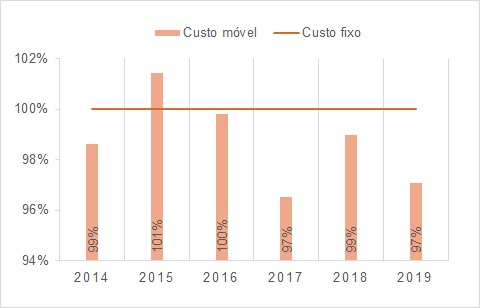
\includegraphics[width=0.7\linewidth]{produtos/prodquatro/custo_comp}
	\caption{Gráfico comparativo dos custos fixos reais com os custos móveis possíveis.}
	\label{fig:custo_comp}
	\legend{Fonte: Elaborado pelos autores.}
\end{figure}
\FloatBarrier

\subsection{Possibilidades na minimização dos custos na prestação dos serviços públicos de limpeza urbana e de manejo de resíduos sólidos em Monteiro Lobato}

A existência de uma série histórica de dados é essencial para que ocorra uma futura análise, um diagnóstico, planejamento de ações e, por fim, melhoria do gerenciamento do processo em questão. 

Tendo em visto o diagnóstico de Monteiro Lobato descrito no Produto 3, salienta-se aqui a importância do registro de dados e monitoramento das atividades diárias voltadas ao resíduo sólido. 

Em Monteiro Lobato, a coleta comum é realizada na segunda, terça, quinta e sexta-feira. Porém, por se tratar de um município de pequeno porte, o Grupo de Acompanhamento desse \gls{pmgirs} informou que nem sempre o caminhão de coleta ocupa a sua carga total e, por isso, não há necessidade de transportar os resíduos ao aterro no municício de Tremembé todo dia em que a coleta é realizada. Dessa forma, é fundamental manter-se um registo constando se a coleta foi realizada de modo completo ou parcial e se ocorreu o deslocamento até Tremembé no mesmo dia. 

Essa fonte de dados impacta diretamente no custo mensal calculado - fixo e móvel, podendo-se alterar os dias de coleta percorridos e os quilômetros percorridos por dia. O diagnóstico realizado no Produto 3 também fica vulnerável à alterações, uma vez que foi realizado um estudo do comportamento de geração de \gls{rsu} comum e reciclável em diversas escalas temporais, inclusive semanal.

O estudo dos custos relacionados ao \gls{rsu} foi viabilizado através de informações disponibilizadas pela secretarias de Monteiro Lobato (tais como o valor salarial dos funcionários ou o rendimento do caminhão compactador de coleta). Mas, principalmente, a análise foi viabilizada através do procedimento da ESTRE-Resicontrol, ao realizar a pesagem do resíduo quando chega em Tremembé.

Tendo em vista tamanha importância, acentua-se a necessidade de replicar o procedimento citado do \gls{rsu} comum para os \gls{rsu} recicláveis (o qual, atualmente, encontra-se sem monitoramento quantitativo e qualitativo).

\newpage
\FloatBarrier
\section{Propostas aplicáveis para redução de resíduos}
%\section{Propostas aplicáveis para redução, reutilização, coleta seletiva e reciclagem de resíduos}

\label{sec:metas}
%% Manual item XIV
%% Entrega 1: 30.nov.2019
%% Autora: Talita Guerra

De acordo com o Diagnóstico Municipal Participativo (Produto 3), uma das fragilidades em relação a consistência de informações que sejam fidedignas à realidade do município é a não identificação e mensuração correta dos dados necessários para inserção na base federal \gls{snis}. A ausência de informações corretas a respeito dos serviços de saneamento pode impedir ou dificultar o conhecimento sobre a situação do município e o planejamento e execução de medidas de controle, mitigação ou solução das questões.

Os formulários de preenchimento do \gls{snis} são muitas vezes extensos porém bastante completos e as informações solicitadas são de conhecimento do município (contratos, registros de operações, folhas de pagamento, etc.).	A partir do preenchimento das informações, o \gls{snis} calcula indicadores de situação que podem ser utilizados para nortear as políticas públicas em relação aos serviços de saneamento básico, dentre eles o gerenciamento de resíduos sólidos, mas esses indicadores somente serão úteis se o município detiver o controle das informações prestadas. 

Em relação aos resíduos sólidos, o município deverá ter clareza da situação da geração e movimentação dos resíduos em seu território (por exemplo: quantidade total de resíduos, quantidade por classe de resíduos, flutuação da quantidade em períodos de alta temporada turística, quantidade de resíduos recicláveis, quantidade de catadores existentes, índice de atendimento de coleta urbana e rural, situação dos caminhões, dentre outras situações) para então planejar e implantar soluções que impactem positivamente na melhoria dos serviços de saneamento e consequentemente na qualidade de vida dos munícipes, tornando a gestão mais eficiente.

Ao se pensar em medidas para a diminuição dos resíduos encaminhados para disposição final ambientalmente adequada, é comum a lembrança da política dos 3Rs relacionados aos resíduos sólidos: redução, reutilização, reciclagem. De fato, a \gls{pnrs}, em seu artigo 9º, estabelece como uma de suas diretrizes a ordem de prioridade na gestão e gerenciamento de resíduos sólidos: a não geração, a redução, reciclagem, o tratamento dos resíduos sólidos e por fim a disposição ambientalmente adequada dos rejeitos. \cite{brasil:12305} Por rejeito entende-se todos os resíduos para os quais não há mais possibilidade de tratamento e recuperação, seja por ausência de tecnologia ou por não ser economicamente viável.

%\textbf{PRINCÍPIOS DA NÃO GERAÇÃO, REDUÇÃO, REUTILIZAÇÃO, RECICLAGEM!!!!}

Como mostrado no Diagnóstico Municipal Participativo (Produto 3), boa parte dos resíduos gerados em Monteiro Lobato são passíveis de aproveitamento, o que os coloca na condição de recursos potenciais, inclusive com geração de renda e não devem, portanto, ter como destino final o aterramento. 

Neste sentido, esta seção do Prognóstico (Produto 4) apresenta algumas propostas que podem ser implantadas no município para promover a redução dos resíduos gerados e atualmente encaminhados para aterro e reaproveitamento de recursos.


\subsection{Redução da quantidade de resíduos sólidos encaminhados para disposição final}

\subsubsection{Segregação na fonte}

Como já abordado anteriormente, a correta segregação dos resíduos gerados na fonte é a principal parte a ser cumprida para a melhoria do manejo de resíduos, incluindo a redução da fração encaminhada para aterro. Logo, estimular todos os setores da sociedade a fazer a correta separação é uma meta que deve ser estimulada durante todo o horizonte de vigência deste plano. 
 
A \autoref{tab:grav_comum_media} traz o resumo da geração de resíduos sólidos comuns a partir da caracterização gravimétrica realizada (Produto 3) para traçar o perfil de geração de resíduos no município. 

%\textbf{\underline{Para que o município consiga atingir as metas para ..... gestão, seguir os indicadores já propostos no Produto 3. Essas metas são.....}}

% Table generated by Excel2LaTeX from sheet 'grav_comum_media'
\begin{table}[htbp]
  \centering
  \caption{Média da composição gravimétrica comum}
	\begin{tabular}{c|c|c|c}
		\rowcolor[rgb]{ .969,  .588,  .275} \textcolor[rgb]{ 1,  1,  1}{\textbf{Tipo de resíduo}} & \multicolumn{1}{p{4.215em}|}{\textcolor[rgb]{ 1,  1,  1}{\textbf{Média}}} & \multicolumn{1}{p{8em}|}{\textcolor[rgb]{ 1,  1,  1}{\textbf{Tipo de resíduo}}} & \multicolumn{1}{p{4.215em}}{\textcolor[rgb]{ 1,  1,  1}{\textbf{Média}}} \\
		\rowcolor[rgb]{ .992,  .914,  .851} \textbf{Orgânico} & 34,10\% & \textbf{Metais mistos} & 5,00\% \\
		\rowcolor[rgb]{ .984,  .831,  .706} \textbf{Tecido} & 12,80\% & \textbf{Madeira} & 2,70\% \\
		\rowcolor[rgb]{ .992,  .914,  .851} \textbf{Higiênicos} & 13,00\% & \textbf{Pneu} & 1,70\% \\
		\rowcolor[rgb]{ .984,  .831,  .706} \textbf{Plástico fino} & 11,40\% & \textbf{Vidro} & 1,40\% \\
		\rowcolor[rgb]{ .992,  .914,  .851} \textbf{Papel/papelão} & 9,90\% & \textbf{Outros} & 1,40\% \\
		\rowcolor[rgb]{ .984,  .831,  .706} \textbf{Plástico duro} & 6,60\% &       &  \\
	\end{tabular}%
  \label{tab:grav_comum_media}%
  \legend{Fonte: Elaborado pelos autores.}
\end{table}%


Pela tabela é possível notar que a segregação na fonte dos resíduos não é corretamente executada, uma vez que se encontra uma parcela considerável (53\%) de materiais que poderiam e deveriam ter outra destinação que não o "lixo" comum. Logo, pensar na redução dos resíduos a serem dispostos passa, além da análise da possibilidade de não gerar o resíduo, mas também pela eficiente segregação na fonte, ou seja, nos domicílios, no comércio, das classes de resíduos. 

Pela \autoref{tab:grav_comum_media} é possível perceber que os munícipes em Monteiro Lobato descartam muitos tecidos na forma de roupas em boas condições de uso. O desvio dessas roupas do aterramento pode ser incentivado através de oficinas de transformação desses tecidos por meio da costura e do artesanato como também a doação dessas roupas a pessoas e entidades que necessitem.  

Já \autoref{tab:grav_seletiva_media} traz o resultado da composição gravimétrica dos resíduos provenientes da coleta seletiva. Novamente observa-se que não há a correta segregação dos resíduos que são destinados à coleta seletiva pois foram encontrados materiais de origem higiênica, o que pode contaminar os resíduos úteis e oferecer risco aos trabalhadores da reciclagem. 

% Table generated by Excel2LaTeX from sheet 'grav_seletiva_media'
\begin{table}[htbp]
  \centering
  \caption{Média da composição gravimétrica seletiva}
	\begin{tabular}{c|c|c|c}
		\rowcolor[rgb]{ .969,  .588,  .275} \textcolor[rgb]{ 1,  1,  1}{\textbf{Tipo de resíduo}} & \textcolor[rgb]{ 1,  1,  1}{\textbf{Média}} & \textcolor[rgb]{ 1,  1,  1}{\textbf{Tipo de resíduo}} & \textcolor[rgb]{ 1,  1,  1}{\textbf{Média}} \\
		\rowcolor[rgb]{ .984,  .831,  .706} \textbf{Papelão} & 40,50\% & \textbf{Higiênicos} & 2,30\% \\
		\rowcolor[rgb]{ .992,  .914,  .851} \textbf{Vidro} & 19,40\% & \textbf{Orgânico} & 2,10\% \\
		\rowcolor[rgb]{ .984,  .831,  .706} \textbf{Plástico duro} & 14,40\% & \textbf{Tetra pak} & 1,30\% \\
		\rowcolor[rgb]{ .992,  .914,  .851} \textbf{Plástico fino} & 10,70\% & \textbf{Metal} & 1,10\% \\
		\rowcolor[rgb]{ .984,  .831,  .706} \textbf{Papel} & 3,80\% & \textbf{Isopor} & 0,50\% \\
		\rowcolor[rgb]{ .992,  .914,  .851} \textbf{Outros} & 2,40\% & \textbf{Tecido} & 1,40\% \\
	\end{tabular}%
  \label{tab:grav_seletiva_media}%
  \legend{Fonte: Elaborado pelos autores.}
\end{table}%


\subsubsection{Resíduos orgânicos}

O tipo de resíduo comum que mais é gerado em Monteiro Lobato é o orgânico e esse tipo de resíduo tem um grande potencial de aproveitamento e é possível transformá-lo em matéria útil dentro das propriedades (rurais e urbanas), sem que seja necessário depender da coleta e destinação desse resíduo. O tratamento dos resíduos orgânicos pode ocorrer de diversas formas. A compostagem é uma dessas formas e de acordo com a Lei de Saneamento Básico (Lei Federal nº 11.445) também é considerada serviço de limpeza urbana e cabe ao titular dos servições de limpeza pública articular para a implantação de sistemas de compostagem.

A compostagem de resíduos orgânicos é a decomposição, na presença de oxigênio, da matéria orgânica dos resíduos de origem animal e vegetal, que têm sua carga orgânica neutralizada e transformada em matéria rica em nutrientes, sem odor e sem potencial poluidor, que podem ser incorporados ao solo tornando-o melhor para o desenvolvimento de plantas e pode ser vinculada a diversos benefícios socioambientais além da redução de resíduos a serem dispostos:

\begin{itemize}
	\item Redução de resíduos para aterramento, consequentemente redução de custos associados e aumento de vida útil do aterro;
	\item Produção de potencial adubo devido a reciclagem de nutrientes;
	\item Uso agrícola do adubo e diminuição dos custos financeiros associados à compra de fertilizantes e diminuição dos custos ambientais inerentes à produção desses fertilizantes;
	\item Diminuição da emissão de CH$_{4}$ (metano) para a atmosfera, gás de elevado potencial de efeito estufa. 
\end{itemize}

Os materiais que podem ser compostados são diversos e geralmente são resíduos orgânicos em geral (domésticos ou não), aparas de grama, resíduos de poda e capina, cinzas e etc, e em geral a montagem de uma composteira, independentemente do tamanho é de uma mistura de parte de resíduo orgânico úmido para partes de matéria seca (serragem, grama seca, lascas de madeira e etc). A atividade pode ser implantada nos municípios desde que haja controle sobre a qualidade dos processos e do produto para que não ocorra a geração de compostos contaminados ou a atividade se torne contaminante do local \cite{felipetto_conceito_2007}. A segregação na fonte é uma das etapas mais importantes do processo de compostagem pois evita que contaminantes como medicamentos, pilhas e outros sejam misturados aos resíduos compostáveis e terminem por prejudicar a qualidade do material final. Por esse motivo é importante conscientizar a população e viabilizar a correta separação dos resíduos compostáveis de outros tipos de resíduos (recicláveis, resíduos de logística reversa, resíduos de construção civil e etc) e dos rejeitos.

Como abordado no Diagnóstico Municipal (Produto 3), cerca de 34 \% dos resíduos da coleta comum no município de Monteiro Lobato são compostos por matéria orgânica que poderia ser compostada, o que diminuiria a contribuição do município tanto em relação a quantidade de resíduos que deixaria de ser aterrada e consequentemente seus próprios custos, quanto a participação na produção de \gls{gee}. Boa parte dos moradores (cerca de 50 \%) já fazem compostagem nos seus espaços próprios, a exemplo de residentes do bairro dos Souzas. O poder público local, focando na gestão participativa, pode buscar manter um diálogo com essas pessoas e comunidades e estabelecer parcerias para troca de informações, métodos e materiais, como equipamentos e matéria seca.

Quando realizado pelos geradores em ambiente domiciliar (no caso, os munícipes) é classificada como compostagem doméstica. Essa forma de compostagem é realizada em recipientes chamados de composteiras ou minhocários, caso sejam utilizadas minhocas no processo. A vantagem da composteira doméstica é que além de diminuir o impacto e os custos inerentes à coleta e destinação desses resíduos, proporciona o tratamento local do resíduo e produz adubo que pode ser utilizado pelo próprio munícipe em seu próprio jardim ou horta. Quando bem feita, não produz odores nem atrai animais vetores de doenças.

A compostagem também pode ser realizada através de Unidades ou Usinas de Compostagem e, neste caso, é uma atividade passível de licenciamento pelo órgão ambiental competente e que necessita ter projeto, implantação e operação bem detalhados e responsáveis técnicos. 

%O Ministério do Meio Ambiente disponibilizou, em 2010, o Manual para implementação de compostagem e de coleta seletiva no âmbito de consórcios públicos. De acordo com esse manual, podem ser implementados...  

%caso a compostagem seja feita pelo município, será necessário ter licença? será necessário atender todos os padrões para fazer adubo? vão doar? qual o custo de implantação? pessoal? treinamento/qualificação? onde poderá ser feito?

Uma das propostas deste plano para incentivar os munícipes na atividade de compostagem é que todos os prédios públicos tenham recipientes próprios para separação do resíduo reciclável do orgânico e também composteiras onde estes resíduos serão dispostos. %META DE CURTO PRAZO. As composteiras podem ser montadadas de diversas formas e de diversos materiais, podendo ser utilizadas minhocas ou apenas micro-organismos.

%\subsection{Reutilização}

\subsection{Traçando um paralelo}
Relacionando as ideias aqui apresentadas aos \gls{ods}, verifica-se que, direta ou indiretamente o manejo adequado dos resíduos pode contribuir para atingir pelo menos 5 dos objetivos:

\begin{itemize}
	\item[\gls{ods} 2] Fome zero e agricultura sustentável. Ao promover a ciclagem de nutrientes, a compostagem fornece adubo para cultivos. Boa parte do território do município de Monteiro Lobato é área rural e passível de plantios; além disso há produtores na região que podem se beneficiar da atividade ao obter adubo de qualidade a preço baixo ou nenhum, caso a atividade seja desenvolvida na propriedade. Plantios próprios podem ajudar as pessoas a ter uma alimentação mais saudável e se corretamente manejados podem contribuir para a preservação do solo, da biodiversidade local, das águas e das tradições culturais alimentares.
	\item[\gls{ods} 4] Educação de qualidade. O item 4.7 fala da educação para o desenvolvimento sustentável e estilos de vida sustentáveis. Repensar e trabalhar a questão dos resíduos em âmbito escolar estimula o desenvolvimento de cidadãos mais conscientes da sua relação com a natureza e o local onde habitam.
	\item[\gls{ods} 6] [Água potável e saneamento]. Garantir a disponibilidade de água de qualidade e em quantidade significa restaurar, manter e proteger os ecossistemas que possibilitam que a água chegue nos cursos d'água. Nesse sentido enriquecer o solo das propriedades com composto para que receba plantios teria como um dos benefícios ajudar a melhorar a qualidade dos recursos hídricos da região. Além disso ao estimular a destinação correta dos resíduos, diminuindo ou mesmo acabando com os pontos de descarte incorreto de resíduos sólidos, diminui-se a poluição decorrente desse descarte e assim também melhora a qualidade das águas da bacia. 
	\item[\gls{ods} 11]	Cidades e comunidades sustentáveis. As soluções para o manejo de resíduos podem ser feitas de forma privada, como soluções individuais, comunitárias, como soluções coletivas ou pelo poder público. De toda forma a diminuição do impacto poluidor dos resíduos e das possibilidades de soluções criativas contribuem para o desenvolvimento de um espaço mais harmonioso e sustentável.
	\item[\gls{ods} 12] Consumo e produção responsáveis. %Resíduos orgânicos, muitas vezes são provenientes do desperdício de alimentos, em toda a cadeia de produção até o consumidor final. 
	Repensar a forma de lidar com o próprio resíduo pode fazer com que as pessoas repensem o consumo que gera o resíduo.  
\end{itemize}

\newpage
\FloatBarrier
\section{Projeções para o horizonte de 20 anos do Plano}
%% Item novo
%% Entrega 1: 30.nov.2019
%% Autora: Talita Guerra
%	https://www.mma.gov.br/estruturas/srhu_urbano/_arquivos/1_manual_elaborao_plano_gesto_integrada_rs_cp_125.pdf


%	https://www.mma.gov.br/cidades-sustentaveis/residuos-solidos/material-t%C3%A9cnico.html

%	http://www.pmf.sc.gov.br/sistemas/pmgirs/arquivos/PMGIRS_CADERNO_3_Prognostico_PMGIRS_Florianopolis.pdf

\begin{comment}
PGRSS para os estabelecimentos geradores de RSS
Descarte específico chapa de raio X
separação de resíduos na ubs 
recipientes rígidos para armazenagem dos resíduos na ubs

novamente, dificuldade para interpretar os dados devido a falta de dados consistentes

cadastro dos geradores de rss
controle dos pesos/volumes/massas dos geradores particulares, por classe de resíduo

rcc - mun: caracterizar grandes e pequenos geradores para facilitar a elaboração PGRCC

pequenos volumes: pev - troca; incentivo a recuperação de móveis (fonte de renda) - coleta e doa

informações de acesso livre

aumentar pontos de coleta de óleo - gerenciar retirada

\end{comment}
\subsection{Projeção populacional: total, urbana, per capta}

A estimativa de crescimento populacional foi feita com base nos dados do Censo de 2010 do \gls{ibge} e utilizando o método geométrico para o crescimento das populações através de uma planilha disponibilizada pelo \gls{mma}. \textbf{\textit{(Planilha MMA)}}  %https://www.mma.gov.br/cidades-sustentaveis/residuos-solidos/material-t%C3%A9cnico.html).

% Table generated by Excel2LaTeX from sheet 'Planilha1'
\begin{table}[htbp]
  \centering
  \arrayrulecolor{white}
  \caption{Projeção da população do município de Monteiro Lobato para o horizonte de 20 anos do Plano}
    \begin{tabular}{c|c|c|c}
    \rowcolor[rgb]{ .969,  .588,  .275} \multicolumn{4}{c}{\textcolor[rgb]{ 1,  1,  1}{\textbf{Projeção populacional}}}\\
    \rowcolor[rgb]{ .984,  .831,  .706} \textbf{Ano} & \textbf{Pop. Urbana} & \textbf{Pop. Rural} & \textbf{Total} \\
    \rowcolor[rgb]{ .992,  .914,  .851} 2020  & 1.983  & 2.482  & 4.465 \\
    \rowcolor[rgb]{ .984,  .831,  .706} 2025  & 2.069  & 2.525  & 4.594 \\
    \rowcolor[rgb]{ .992,  .914,  .851} 2030  & 2.139  & 2.544  & 4.683 \\
    \rowcolor[rgb]{ .984,  .831,  .706} 2035  & 2.193  & 2.544  & 4.737 \\
    \rowcolor[rgb]{ .992,  .914,  .851} 2040  & 2.228  & 2.518  & 4.746 \\
    \end{tabular}%	
  \label{tab:proj_pop}%
  \legend{Fonte: Fundação Seade.}
\end{table}%


Caso a projeção populacional se confirme, Monteiro Lobato terá um acréscimo de aproximadamente 1.400 pessoas que devem contribuir para o aumento da geração de resíduos sólidos no município. Importante ressaltar que o próximo Censo do \gls{ibge} deverá ocorrer em breve e gerar dados populacionais mais próximos da realidade municipal, que podem diferir da projeção, ainda assim, a projeção é muito útil para fins de planejamento futuro.

\subsection{Projeção da geração de resíduos totais}

\subsubsection{Cenário tendencial}

As projeções foram feitas para o cenário tendencial pelo método geométrico para as classes de resíduos para as quais o município dispõe de dados, que são os resíduos comuns e os resíduos de serviços de saúde coletados por empresa terceirizada. 

%\input{./produtos/prodquatro/proj_residuos.tex}

As taxas per capta de geração de resíduos foram estimadas pelas médias de geração do período entre 2014 e 2017. 

Para o resíduo comum, considerando o aumento populacional, a quantidade de resíduos gerados e que teriam como destino o aterro sanitário teria um acréscimo de aproximadamente 200 toneladas, o que daria um acréscimo anual de 10 toneladas a cada ano, até 2040, como mostra a \autoref{fig:projrscomum}.

 \begin{figure}[h]
 	\centering
 	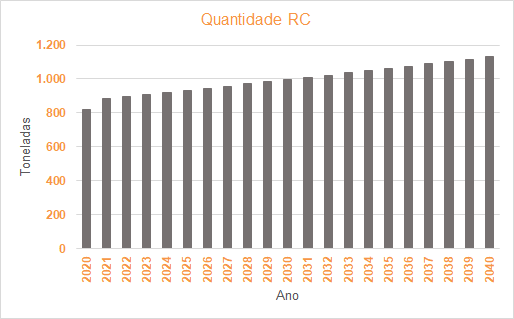
\includegraphics[width=0.7\linewidth]{produtos/prodquatro/proj_rs_comum}
 	\caption{Projeção para os resíduos comuns de Monteiro Lobato}
 	\label{fig:projrscomum}
 \end{figure}

Os dados dos resíduos de saúde foram estimados com base na quantidade de resíduos recolhida pela empresa especializada AGIT Soluções Ambientais Ltda para o período. Os resíduos de saúde são classificados em 5 categorias %(seção xxxxx P3) 
e a coleta realizada pela empresa Soluções Ambientais Ltda ocorre para os grupo de resíduos A e E. Os outros grupos são recolhidos pela coleta comum e não são quantificados, de modo que não há informações detalhadas sobre eles. A \autoref{fig:projrss} traz a projeção do \gls{rss}.

\begin{figure}[h]
	\centering
	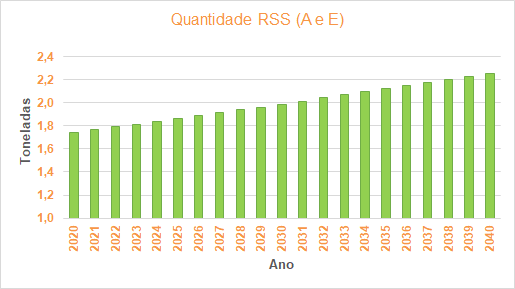
\includegraphics[width=0.7\linewidth]{produtos/prodquatro/proj_rss}
	\caption{Projeção dos resíduos do serviço de saúde para Monteiro Lobato}
	\label{fig:projrss}
\end{figure}

Analisando a projeção, é possível estimar um aumento da geração de \gls{rss} que ultrapassaria, em 2023, a quantidade atualmente contratada de 1,8 tonelada anual de resíduo a ser coletada e disposta pela empresa especializada, ademais, os outros grupos de resíduos de \gls{rss} (B, C, E) recolhidos pela coleta comum também devem aumentar significando elevação custos para essa classe. O grupo de resíduos D geralmente é composto por resíduos passíveis de reciclagem e representa uma grande porção do total (75\% a 90\%) gerado em locais de serviços de saúde (MMA, 2011), logo, a correta segregação e destinação adequada desse grupo pode significar recuperação de parte dos recursos graças à reciclagem.   

Para ambas as classes de resíduos projetadas, verificou-se o aumento da geração e, caso mantidas as condições atualmente praticadas no município, os custos com transporte, armazenamento e disposição desses resíduos deve aumentar. 
%\subsubsection{Cenário Planejado}	Com aplicação do Plano

\newpage
\FloatBarrier
\section{Descrição das formas e limites da participação do poder público local na coleta seletiva, na logística reversa e de outras ações relativas à responsabilidade compartilhada pelo ciclo de vida dos produtos}
\label{sec:lim_poder_pub}
%% Manual item XV
%% Entrega 1: 30.nov.2019
%% Autora: Laís Shiki

O Art. 30° da Lei Federal 12.305/2010 institui a responsabilidade compartilhada pelo ciclo de vida dos produtos, que segundo tal artigo deve ser implementada de forma individualizada e encadeada, abrangendo os fabricantes, importadores, distribuidores e comerciantes, os consumidores e os titulares dos serviços públicos de limpeza urbana e de manejo de resíduos sólidos. Essa responsabilidade compartilhada possui como objetivos: \cite{brasil:12305} 

\begin{itemize}
	\item Compatibilizar interesses entre os agentes econômicos e sociais e os processos de gestão empresarial e mercadológica com os de gestão ambiental, desenvolvendo estratégias sustentáveis;
	\item Promover o aproveitamento dos resíduos sólidos, direcionando-os para a sua cadeia produtiva ou para outras cadeias produtivas;
	\item Reduzir a geração de resíduos sólidos, o desperdício de materiais, a poluição e os danos ambientais;
	\item Incentivar a utilização de insumos de menor agressividade ao meio ambiente e de maior sustentabilidade;
	\item Estimular o desenvolvimento de mercado, a produção e o consumo de produtos derivados de materiais reciclados e recicláveis;
	\item Propiciar que as atividades produtivas alcancem eficiência e sustentabilidade;
	\item Incentivar as boas práticas de responsabilidade socioambiental.    
\end{itemize}

Cabe a este \gls{pmgirs}/Monteiro Lobato descrever as formas e limites da participação do poder público municipal na coleta seletiva e na logística reversa, obedecendo a \gls{pnrs} e outras legislações pertinentes ao assunto. 

\subsection{Coleta seletiva}

Implementar a coleta seletiva é essencial para atingir a meta de disposição final ambientalmente adequada dos rejeitos, segundo o Art. 9°, parágrafo um do Decreto Federal nº 7.404/2010. A Prefeitura de Monteiro Lobato já possui um sistema de coleta seletiva, que realiza coleta uma vez por semana e abrange toda a área urbana e rural do município. Na \autoref{sec:educ_amb} são propostas oficinas e ações que irão conscientizar e incentivar os munícipes e servidores públicos em relação a este sistema. 

Novamente no Art. 9° do Decreto Federal nº 7.404/2010, o parágrafo dois estabelece que a coleta seletiva deverá ser implantada pelo titular do serviço público de limpeza urbana e manejo de resíduos sólidos. Porém, o poder público local deve desenvolver ações e metas para dar continuidade na efetividade e aprimoramento do sistema de coleta seletiva. Para tanto, na \autoref{tab:limites_coleta_seletiva} são listadas algumas medidas cabíveis. 

% Table generated by Excel2LaTeX from sheet 'limites_coleta_seletiva'
\begin{table}[htbp]
  \centering
  \caption{Descrição das formas e limites da participação do poder público local na coleta seletiva}
    \begin{tabular}{P{40.855em}}
    \rowcolor[rgb]{ .992,  .914,  .851} Implantar e operar um LEV para entrega voluntária de recicláveis \\
    \rowcolor[rgb]{ .984,  .831,  .706} Estabelecer a forma correta de segregação dos RD e RC \\
    \rowcolor[rgb]{ .992,  .914,  .851} Determinar os procedimentos para o acondicionamento e descarte adequado dos materiais recicláveis \\
    \rowcolor[rgb]{ .984,  .831,  .706} Incentivar a população a realizar às boas práticas em relação a coleta seletiva \\
    \rowcolor[rgb]{ .992,  .914,  .851} Criar e priorizar a participação de cooperativas ou outro tipo de associação de catadores constituídas por pessoas físicas de baixa renda \\
    \rowcolor[rgb]{ .984,  .831,  .706} Capacitar os servidores públicos e atores sociais envolvidos na coleta seletiva \\
    \rowcolor[rgb]{ .992,  .914,  .851} Disponibilizar lixeiras específicas para cada tipo de material reciclável em pontos estratégicos no município \\
    \rowcolor[rgb]{ .984,  .831,  .706} Formentar a implementação de soluções consorciadas ou compartilhadas com municípios vizinhos \\
    \end{tabular}%
  \label{tab:limites_coleta_seletiva}%
  \legend{Fonte: Elaborado pelos autores, adaptado da PNRS (2010).}
\end{table}%


O poder público de Monteiro Lobato pode criar incentivos econômicos para os consumidores que participam da coleta seletiva, na forma de lei municipal, de acordo com o Art. 35 da \gls{pnrs}. Todavia, os consumidores possuem as seguintes obrigatoriedades:

\begin{itemize}
	\item Acondicionar adequadamente e de forma diferenciada os resíduos sólidos gerados; 
	\item Disponibilizar adequadamente os resíduos sólidos reutilizáveis e recicláveis para coleta ou devolução.    
\end{itemize}

\subsection{Logística reversa}
\label{subsec:desc_lr}

Os fabricantes, importadores, distribuidores e comerciantes de produtos obrigados a estruturar e implementar uma cadeia de logística reversa, citados na \autoref{sec:rs_geradores_lr}, devem fazer isto de forma independente do serviço público de limpeza urbana e de manejo dos resíduos sólidos \cite{brasil:12305}. Porém, é interessante o poder público local realizar certas medidas a fim de incentivar e/ou facilitar a efetivação desses sistemas. Na \autoref{tab:limites_log_reversa} são descritas algumas formas e limites para o poder público atuar nestes casos.


% Table generated by Excel2LaTeX from sheet 'limites_log_reversa'
\begin{table}[htbp]
	\centering
	\caption{Descrição das formas e limites da participação do poder público local na logística reversa}
	\begin{tabular}{P{40.855em}}
		\rowcolor[rgb]{ .992,  .914,  .851} Identificar os resíduos e seus geradores sujeitos ao sistema de logística reversa \\
		\rowcolor[rgb]{ .984,  .831,  .706} Incentivar o setor privado para a estruturação de acordos setoriais, com vista à implementação ou expansão da logística reversa \\
		\rowcolor[rgb]{ .992,  .914,  .851} Prever a participação de entidades, cooperativas de catadores ou outras formas de associações constituídas por pessoas de baixa renda na estruturação de acordos setoriais \\
		\rowcolor[rgb]{ .984,  .831,  .706} Celebrar termos de compromisso junto aos fabricantes, distribuidores e/ou comércios, visando à implantação ou expansão da logística reversa \\
		\rowcolor[rgb]{ .992,  .914,  .851} Implantar a logística reversa via promulgação de regulamentos normativos veiculados por Decreto editado pelo Poder Executivo, exigindo e fiscalizando a sua efetividade \\
		\rowcolor[rgb]{ .984,  .831,  .706} Exigir que todos os atores envolvidos no sistema de logística reversa disponibilizem informações completas sobre a realização de suas ações, com periodicidade semestral  \\
		\rowcolor[rgb]{ .992,  .914,  .851} Articular, coordenar, promover e supervisionar programas de educação ambiental com foco na logística reversa \\
		\rowcolor[rgb]{ .984,  .831,  .706} Articular com os fabricantes no sentido de implantar sistemas de logística reversa, bem como difundir tais programas \\
		\rowcolor[rgb]{ .992,  .914,  .851} Manter sistemas de logística reversa implementados em entidades e/ou instituições públicas \\
		\rowcolor[rgb]{ .984,  .831,  .706} Garantir a continuidade e permanência do processo educativo \\
		\rowcolor[rgb]{ .992,  .914,  .851} Fiscalizar o descarte ambientalmente correto dos resíduos sujeitos à logística reversa \\
	\end{tabular}%
	\label{tab:limites_log_reversa}%
	\legend{Fonte: Elaborado pelos autores, adaptado do PMGIRS/Arujá (2018)}
\end{table}%


\FloatBarrier


A fim de implementar e operacionalizar os sistemas de logística reversa, a \gls{pnrs} define os seguintes instrumentos: regulamentos, acordos setoriais e termos de compromisso, os dois últimos a serem firmados entre o poder público e o setor empresarial. Os acordos setoriais são “atos de natureza contratual, firmados entre o Poder Público e os fabricantes, importadores, distribuidores ou comerciantes, visando à implantação da responsabilidade compartilhada pelo ciclo de vida do produto” \cite{brasil:12305}. Já os termos de compromisso, ainda segundo a  \gls{pnrs}, podem ser assinados somente nos casos onde não houver acordo setorial ou regulamento específico com a mesma abrangência geográfica ou para estabelecer metas e compromissos mais exigentes que os previstos nos acordos ou regulamentos.


\newpage
\section{Meios a serem utilizados para controle e fiscalização, no âmbito local, da implementação e operacionalização dos planos de gerenciamento de resíduos sólidos e dos sistemas de logística reversa}
\label{sec:meios_controle_fisc}
%% Manual item XVI
%% Entrega 2: 13.nov.2019
%% Autora: Laís Shiki

Na \autoref{sec:rs_geradores_lr} foi identificado os resíduos sólidos e geradores que estão sujeitos ao \gls{pgrs} ou ao sistema de logística reversa em Monteiro Lobato. Neste sentido, este tópico visa propor algumas ações e indicadores para acompanhar, controlar e fiscalizar tais agentes.

Uma das ações recomendadas, para o poder público local, é a de estimar a quantidade de resíduos sujeitos ao plano de gerenciamento ou ao sistema de logística reversa.  Assim, como manter atualizado o levantamento destes geradores, é recomendado conter neste levantamento os seguintes dados: \cite{agevap_manual_2019}

\begin{itemize}
	\item Identificação do gerador: razão social, CNPJ, descrição da atividade, responsável legal, entre outras;
	\item Identificação dos resíduos gerados: resíduo, classificação, acondicionamento e/ou armazenagem, frequência de geração, entre outros; 
	\item Plano de movimentação dos resíduos: tipo de resíduo, quantidade, local de estocagem temporário (se for o caso), transporte a ser utilizado, destinação final, entre outros;
	\item Indicador de coleta: relação entre quantidade de material coletado e a quantidade de material gerado;
	\item Indicador de rejeito: relação entre o rejeito acumulado e o material recebido para tratamento.
\end{itemize}

É necessário que o município realize a cobrança do \gls{pgrs}, estipulando prazo máximo a sua entrega e penalidades caso ocorra atraso ou não execução. Vale ressaltar que aqueles que devem elaborar o \gls{pgrs} são obrigados a disponibilizar e manter atualizadas todas informações sobre a implementação e operacionalização do plano ao órgão municipal competente \cite{brasil:12305}. 

Como foi apontado no Produto 3 (Diagnóstico Municipal Participativo) deste \gls{pmgirs}, há certas irregularidades em relação ao sistema de logística reversa no município. Logo, convocar uma reunião de caráter obrigatório com comerciantes e outros envolvidos com produtos sujeitos a realizar a logística reversa, a fim de conscientizar estes sobre a importância de se elaborar o \gls{pgrs}, seria de demasiada importância. 

Utilizar os indicadores propostos no subtópico 2.6 do Produto 3 deste plano, por exemplo os indicadores para \gls{rss}, \gls{rcc} e \gls{ra}, é um meio de controlar e consequentemente fiscalizar os planos de gerenciamento e os sistemas de logística reversa.



\FloatBarrier
\newpage
\section{Ações preventivas e corretivas}
\label{sec:acoes_prev_corr}
%% Manual item XVII
%% Entrega 2: 13.nov.2019
%% Autora: Lia Yukari

Este capítulo pretende descrever as medidas preventivas e corretivas a serem adotadas pelo município quanto ao gerenciamento dos resíduos sólidos, denotando as preventivas como aquelas medidas necessárias a evitar que um problema potencial se materialize e as corretivas as ações que convergem para que um problema existente não
tenha recorrência e/ou que seu impacto seja mitigado e/ou até revertido conforme possibilidades aplicáveis ao caso concreto \cite{pmgirs_aruja3_2018}.

Qualquer atividade realizada, mesmo que planejada, está sujeita à imprevisibildades; para isso, elaborou-se nesse presente produto a \autoref{sec:emerg_corr}. As ações aqui descritas, de prevenção e correção, têm a intenção de minimizar essas ocorrências através de medidas protocoladas dentro do município em questão.

As ações preventivas e corretivas referentes ao município de Monteiro Lobato já foram descritas no Produto 3 desse presente \gls{pmgirs}, cabe ao Produto 4 delimitar os pontos práticos a serem planejados no município a fim de se concretizar tais ações de modo mais eficiente. A \autoref{tab:acoes_prevent} mostra os pontos a serem planejados e colocados em prática no município.

% Table generated by Excel2LaTeX from sheet 'acoes_prevent'
\begin{table}[htbp]
	\centering
	\caption{Ações preventivas e corretivas do município de Monteiro Lobato.}
	\resizebox{\textwidth}{!}{%
    \begin{tabular}{p{18em}p{7.91em}p{21.545em}p{21.545em}}
	\rowcolor[rgb]{ .969,  .588,  .275} \textcolor[rgb]{ 1,  1,  1}{\textbf{AÇÃO}} & \textcolor[rgb]{ 1,  1,  1}{\textbf{PRVENTIVA (P) CORRETIVA (C)}} & \textcolor[rgb]{ 1,  1,  1}{\textbf{DIAGNÓSTICO}} & \textcolor[rgb]{ 1,  1,  1}{\textbf{PROGNÓSTICO}} \\
	\rowcolor[rgb]{ .992,  .914,  .851} Controle de emissão de gases e percolados & P     & Existente. Atualmente a disposição final dos resíduos sólidos ocorre no aterro sanitário de Tremembé, dotado de sistema de drenagem e correto tratamento/destinação dos gases e percolados, de maneira a prevenir possíveis impactos advindos dos mesmos. & Fazer frequentemente o monitoramente do aterro sanitário em que são enviados os resíduos sólidos, quanto ao licenciamento exigido pelo seu respectivo Órgão Ambiental. Analisar previamente a existência de um protocolo legal caso os resíduos sólidos passem a ser dispostos em um novo local. \\
	\rowcolor[rgb]{ .984,  .831,  .706} Educação ambiental para redução e reaproveitamento de resíduos nas fontes geradoras & P     & Existente. Nas redes de ensino. O Instituto Pandavas, localizado no Bairro do Souza, é um dos principais centros pedagógicos atuantes na região. & Tornar uma ação de caráter também corretivo. Ampliar para todas as redes de ensino, instituições, empresas e comércio. Seguir aplicação de ações propostas na \autoref{sec:educ_amb}. \\
	\rowcolor[rgb]{ .992,  .914,  .851} Coleta seletiva e triagem dos resíduos & P     & Indefinido no período de elaboração desse produto. A coleta setetiva e sua triagem evita que parte dos resíduos secos recicláveis sejam destinados aos aterros sanitários. & Seguir diretrizes da \autoref{sec:capac_tec} e \autoref{sec:metas}. Melhorar a eficiência do programa de coleta seletiva. Transmitir conscientização à população quanto a separação dos resíduos recicláveis. Contar com dispositivos de entrega dos resíduos secos, como em \gls{lev}. Estabeleber um termo contratual com algum local de destinação de resíduos recicláveis. Viabilizar, antecipadamente, um termo de renovação ou uma nova associação. Levantar um cadastro de locais passíveis a receberem resíduos recicláveis em caso de emergência. \\
	\rowcolor[rgb]{ .984,  .831,  .706} Entrega voluntária de resíduos & P     & Existente. Para óleos de cozinha, evitando a destinação incorreta. Os dois pontos de entrega ocorrem através de bombonas de 50 litros e localizam-se próximos ao Terminal Rodoviário e na Secretária de Meio Ambiente e Agricultura. & Aumentar a diversidade, capacidade e abrangência dos \gls{lev} e Ecopontos a serem instalados no município, visando aumentar o atendimento à população. Realizar programas para sensibilizar a população da importância da entrega voluntária dos resíduos produzidos. \\
	\rowcolor[rgb]{ .992,  .914,  .851} Manutenção preventiva de frota e equipamentos utilizados nos serviços de limpeza e disposição final de resíduos & P/C   & Inexistente. A existência de manutenção preventiva da frota e dos equipamentos utilizados no sistema de limpeza urbana e manejo de resíduos sólidos evita situações de paralização dos serviços. & Realizar revisão preventiva nos caminhões com vistas a evitar interrupções na prestação de serviço devido a problemas mecânicos. Possuir veículos reserva os opcões pré-estabelecidas de empréstimo a fim de garantir que a prestação dos serviços de coleta e disposição final de resíduos não seja afetada por problemas na frota e interrupção da circulação de um dos caminhões. Ter disponibilidade de mecânico para realizar as manutenções necessárias e/ou convênio com alguma oficina mecânica que preste este tipo de serviço periodicamente. \\
	\rowcolor[rgb]{ .984,  .831,  .706} Programa de monitoramento da eficiência dos serviços de coleta e limpeza publica & P/C   & Inexistente. Identifica problemáticas decorrentes das estruturas e serviços, possibilitando seus devidos diagnósticos e correções, acarretando em uma maior eficiência dos serviços. & Seguir diretrizes da \autoref{sec:proc_oper}, \autoref{sec:capac_tec}, \autoref{sec:grup_int} e\autoref{sec:metas}. \\ 
	\rowcolor[rgb]{ .992,  .914,  .851} Programa de monitoramento da eficiência da disposição final de resíduos sólidos & P/C   & Inexistente. O aterro de disposição (Tremembé) contabiliza a quantidade de resíduo recebida e aterrada, porém, o município não monitora as devidas quantidades, a fim de se obter uma maior eficiência. & Seguir diretrizes da \autoref{sec:capac_tec} e \autoref{sec:metas}. Melhorar a eficiência do programa de coleta comum. Transmitir conscientização à população quanto a separação dos resíduos comuns e orgânicos. Monitorar as quantidades de resíduo aterrada por mês, tanto como catalogá-los no \gls{snis}. Viabilizar, antecipadamente, um termo de renovação com o atual local de disposição final ou uma nova associação. Levantar um cadastro de locais passíveis a receberem resíduos comuns em caso de emergência. \\
	\rowcolor[rgb]{ .984,  .831,  .706} Programa de monitoramento de descarte de RCC & P/C   & Inexistente. Identifica problemáticas decorrentes das estruturas e serviços, possibilitando seus devidos diagnósticos e correções, acarretando em uma maior eficiência dos serviços. & Regularizar um local de destinação correta dos \gls{rcc}, através de um bota fora. Realizar o controle do \gls{rcc} e seu respectivo local de acordo com a \autoref{subsec:trans_rcc}. \\
	\rowcolor[rgb]{ .992,  .914,  .851} Programa de monitoramento de geradores de Logística Reversa & P/C   & Inexistente. Identifica problemáticas decorrentes das estruturas e serviços, possibilitando seus devidos diagnósticos e correções, acarretando em uma maior eficiência dos serviços. & Garantir a funcionalidade da logística reversa através de um monitoramento de seus geradores, levantados no Produto 3. Seguir diretrizes estabelecidas na \autoref{subsec:desc_lr}. \\
	\rowcolor[rgb]{ .984,  .831,  .706} Levantamento dos geradores sujeitos aos planos de gerenciamento de resíduos sólidos e ao estabelecimento de sistemas de logística reversa. & P     & Existente. O cadastro foi realizado para a elaboração do diagnóstico do PMGIRS. Facilita a fiscalização contribuindo para que sejam evitadas práticas incorretas e consequentemente prevenindo impactos adversos decorrentes do inadequado manejo dos resíduos sólidos. & Garantir a funcionalidade da logística reversa através de um monitoramento de seus geradores, levantados no Produto 3. Seguir diretrizes estabelecidas na \autoref{subsec:desc_lr}. \\
	\rowcolor[rgb]{ .992,  .914,  .851} Cadastro de aterros próximos para uma possível recepção dos resíduos comuns em caso de impeditivo de disposição final no local atualmente utilizado & P     & Há o conhecimento acerca dos empreendimentos existentes passíveis de atender o município, podendo ser uma alternativa em caso de necessidade, mas não há contratos emergenciais pré-estabelecidos. & Estabelecer contratos emergenciais conforme descritos em \autoref{sec:emerg_corr}. Fazer uso das diretrizes estabelecidas na \autoref{sec:sol_cons} e na \autoref{sec:grup_int}. \\
	\rowcolor[rgb]{ .984,  .831,  .706} Cadastro de empresas que prestam serviços de limpeza, coleta e disposição final de resíduos como opção de contratos emergenciais para suprir uma ausência não prevista dos serviços & P     & Há o conhecimento acerca das empresas existentes passíveis de atender o município, podendo ser uma alternativa em caso de necessidade, mas não há contratos emergenciais pré-estabelecidos. & Estabelecer contratos emergenciais conforme descritos em \autoref{sec:emerg_corr}. Fazer uso das diretrizes estabelecidas na \autoref{sec:sol_cons} e na \autoref{sec:grup_int}. \\
\end{tabular}%
}
	\label{tab:acoes_prevent}%
	\legend{Fonte: Elaborado pelos autores, adaptado do PMGIRS/Arujá (2018).}
\end{table}%

\FloatBarrier

\newpage
\section{Identificação dos passivos ambientais relacionados aos resíduos sólidos e medidas saneadoras}
\label{sec:passivos_amb}
%% Manual item XVIII
%% Entrega 2: 13.nov.2019
%% Autora: Lia Yukari

Passivos ambientais são os custos (financeiros, econômicos, sociais, entre outros) necessários para preservar, recuperar e proteger o meio ambiente. A identificação do passivo ambiental diz respeito não só à sanção a ser aplicada por um dano já realizado ao meio ambiente, mas também a medidas de prevenção de danos ambientais que têm reflexos econômico-financeiros \cite{agevap_manual_2019}.

Alguns passivos ambientais relacionados aos resíduos sólidos são: Contaminação de áreas, inclusive lixões e aterros controlados; Emissão de gases; Contaminação de águas superficiais e subterrâneas \cite{agevap_manual_2019}.

\subsection{Resíduo Sólido Urbano (RSU)}
Em Monteiro Lobato, ocorre atualmente a disposição final adequada do \gls{rsu} em aterro sanitário com controle de emissão de gases e percolado. De qualquer forma, é sempre cabível ao município a aplicação da \autoref{sec:metas} (Metas de redução, reutilização, coleta seletiva e reciclagem) para minimizar seu impacto no aterro sanitário de destinação.

Salienta-se que, mesmo que o aterro sanitário de Tremembé esteja dentro das condições legalmente exigidas, ou não esteja localizado dentro do município de Monteiro Lobato (onde os resíduos são gerados), cabe ao município a minimização de seu impacto até a disposição final. Isso é, uma vez que os aterros sanitários contam com uma vida útil limitada, o município pode e deve reduzir ao máximo o volume a ser destinado, através de campanhas de reutilização e conscientização de separação dos recicláveis.

Ademais, a lavagem dos caminhões de \gls{rsu} (comum e reciclável) deve ser realizada de forma a não contaminar as águas superficiais e subterrâneas, sendo aderida ao sistema de esgotamento sanitário. Deve-se tomar cuidado quanto à superfície que é atingida pela água contaminada de lavagem e à rota de escoamento do mesmo, até atingir a macro drenagem.


\subsection{Resíduo de Construção Civil (RCC)}
Tratando-se do \gls{rcc}, como descrito no Produto 3 e na \autoref{subsec:trans_rcc} desse Produto 4, a disposição do mesmo não é realizada de maneira adequada. Os \gls{rcc} são armazenados ao ar livre no pátio da prefeitura no bairro Morada do Sol,  onde observa-se a disposição inadequada dos resíduos em solo exposto e ao ar livre, sendo utilizados em estradas vicinais e nas valetas e buracos com erosões, quando necessário. A \autoref{fig:patio_rcc} e a \autoref{fig:rcc} mostram, respectivamente, o local e um ponto onde ocorre essa irregularidade.

\begin{figure}[h]
	\centering
	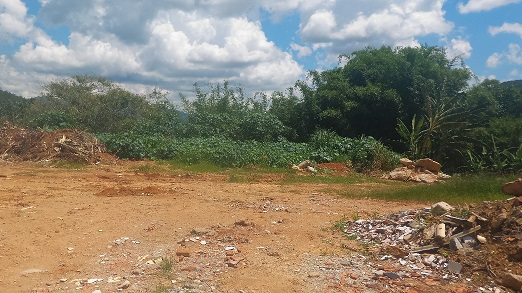
\includegraphics[width=0.7\linewidth]{produtos/prodquatro/patio_rcc}
	\caption{Pátio da Prefeitura onde são dispostos os \gls{rcc}}
	\label{fig:patio_rcc}
	\legend{Fonte: Elaborado pelos autores.}
\end{figure}

\begin{figure}[h!]
	\centering
	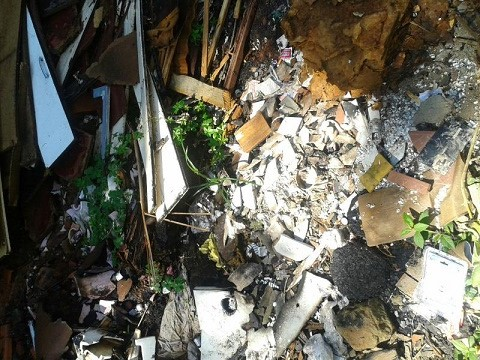
\includegraphics[width=0.6\linewidth]{produtos/prodquatro/rcc}
	\caption{Disposição inadequeda dos \gls{rcc}}
	\label{fig:rcc}
	\legend{Fonte: Elaborado pelos autores.}
\end{figure}

Dessa forma, é importante estabelecer as diretrizes propostas na \autoref{subsec:trans_rcc}, cumprindo também o papel de ação preventiva e corretiva (\autoref{tab:acoes_prevent}) desse tipo de resíduo quanto à contaminação do solo, das águas pluviais, à dispersão de vetores ou de particulados

\FloatBarrier
\newpage
\section{Periodicidade da revisão do PMGIRS}
\label{sec:revisao_pmgirs}
%% Manual item XIX
%% Entrega 3: 26.nov.2019
%% Autora: Lia Yukari

Consoante com a Lei Federal nº 12.305 de 2010, o \gls{pmgirs} deve ser revisado periodicamente, de preferência acompanhando o período de vigência do \gls{ppa} municipal. Assim, as ações estabelecidas no Plano poderão ser aprovadas e contempladas dentro dos recursos previstos no \gls{ppa} de Monteiro Lobato.

O \gls{ppa} vigente no município durante a elaboração desse Plano corresponde a Lei nº 1.657 de 2017, referente ao quadriênio de 2018 a 2021. Assim, os próximos quadriênios serão contidos dentro dos períodos:

\begin{itemize}
	\item 2022/2025
	\item 2026/2029
	\item 2030/2033
	\item 2034/2037
\end{itemize}

A deliberação do \gls{ppa} é realizada na iminência de entrada do próximo quadriênio, assim, recomenda-se que o \gls{pmgirs} seja revisto nos anos 2025, 2029, 2033 e 2037.

As projeções, ações e metas contidas nesse \gls{pmgirs} (com previsão de publicação em 2020) possuem um horizonte de 20 anos. Desse modo, em 2040 faz-se necessária a atualização desse instrumento legal de gestão dos resíduos sólidos.

\FloatBarrier
\newpage
\section{Ações para mitigação das emissões dos gases de efeito estufa}
\label{sec:acoes_efeito_estufa}
%% Manual item XX
%% Entrega 2: 13.nov.2019
%% Autora: Maysa Rocha
Segundo o relatório de Estimativas Anuais de Emissões de Gases do Efeito Estufa, realizado pelo Ministério da Ciência, Tecnologia e Inovação (2013), em 2010 o setor de disposição de resíduos sólidos e o tratamento de efluentes foi responsável por cerca de 4 \% das emissões nacionais de GEE’s.
Sendo que, as variações percentuais acumuladas no período de 2005 a 2010 mostram que as emissões desse setor cresceram a uma taxa superior a 16 \%, representando um importante setor em termos de potencial de redução de emissão

A sessão 5 do produto 3 discorre sobre a definição dos gases do efeito estufa e de forma sucinta aborda algumas ações como proposta para o município mitigar a geração dos gases do efeito estufa. 

\textbf{Rotas de coleta}
O itinerário de coleta é o trajeto que o veículo coletor deve percorrer dentro de um mesmo setor, num mesmo período, transportando o máximo de lixo num mínimo de percurso improdutivo, com o menor desgaste possível para a guarnição e o veículo. Dá-se o nome de percurso improdutivo aos trechos em que o veículo não realiza coleta, servindo apenas para o deslocamento de um ponto a outro.\cite{dalmeida_manual_2018}

Para traçar uma rota de coleta é necessário estudar alguns aspectos do meio físico da região, como por exemplo o relevo, a geomorfologia, o uso e ocupação do solo. A rota de coleta precisa ser eficiente para que percorra o menor caminho e recolha a maior quantidade de resíduos dispostos. É de suma importância pois além de diminuir gastos desnecessários com combustível, reduz a emissão de gases do efeito estufa.

\textbf{Doação de mudas}
De acordo com o relatório divulgado pela Indústria Brasileira de Árvores (Ibá), o plantio de mudas traz vantagens para o meio ambiente, principalmente no combate ao aumento da concentração dos gases do efeito estufa.
A compensação por meio de plantios florestais é uma forma
natural de sequestrar o gás carbônico pelos vegetais
através da fotossíntese, fixando-o em forma de matéria
lenhosa ou biomassa. O sequestro de carbono constitui o
processo de crescimento dos vegetais, ou seja, quanto
maior o porte da planta, mais biomassa se acumula e,
consequentemente, maior é a quantidade de carbono fixada \cite{changman_sequestroc_2004} 
Portanto, incentivar o plantio de mudas ou a doação de mudas é uma iniciativa que beneficia diretamente o meio ambiente e reduz as emissões dos gases do efeito estufa.


\textbf{Aumentar a fiscalização da queima de resíduos}
Embora, em termos globais, a queima de combustíveis fósseis (na produção de energia, nos processos industriais e nos transportes) seja a principal fonte de GEE, responsáveis pelas alterações no clima, os resíduos sólidos têm um papel importante nesse cenário, uma vez que também contribuem para a emissão desses gases \cite{IPCC_2008} . O gerenciamento inadequado dos resíduos sólidos urbanos gera diretamente outros impactos importantes, tanto ambientais quanto na saúde da população. \cite{WHO_Europe_2007}

Há também a emissão de partículas e outros poluentes atmosféricos, diretamente pela queima de lixo ao ar livre ou pela incineração de dejetos sem o uso de equipamentos de controle adequados. De modo geral, os impactos dessa degradação estendem-se para além das áreas de disposição final dos resíduos, afetando toda a população.\cite{Gouveia_riscogee_2010}

Com isso, uma proposta para erradicar a queima de resíduos sólidos  seria aumentar ou firmar a fiscalização nas ruas, em terrenos baldios para que isso não ocorra, pois a toxicidade dos gases  traz danos à saúde da população e colabora para poluição do ar.

\textbf{Redução do resíduo orgânico}
Segundo \cite{Inacio2010} a compostagem por processo aeróbico gera baixas quantidades de metano por tonelada de resíduos orgânicos em comparação com formas de tratamento anaeróbio ou disposição em aterro. Desta forma, a compostagem de resíduos apresenta grande potencial como estratégia de mitigação das emissões de metano, mesmo no contexto de amplos sistemas de gestão de resíduos urbanos, agrícolas ou agroindustriais.
Com isso, os resíduos orgânicos biodegradáveis que normalmente são dispostos inapropriadamente e são decompostos de forma anaeróbica (emissão de GEE’s), seriam tratados em um sistema aeróbio (compostagem). O uso de composto orgânico pode reduzir a dependência do uso de fertilizantes nitrogenados, que são responsáveis pela emissão de N$_{2}$O, que possui GWP(Potencial de aquecimento global) 310 vezes maior ao do CO$_{2}$. \cite{IPCC_2008}
Além da compostagem, "o município de Monteiro Lobato pode incentivar a população e os restaurantes da cidade a não desperdiçarem alimentos nas refeições, evitando sobras e utilizar todos os componentes dos mantimentos que normalmente são jogados fora, como casca, talos" e folhas, como discorre a sessão 5 do Produto 3.


\FloatBarrier
\newpage
\section{Ações para emergência e contingência}
\label{sec:emerg_corr}
%% Manual item XXI
%% Entrega 2: 13.nov.2019
%% Autora: Maysa Rocha

A Seção 6 do produto 3 aborda toda a parte teórica e a definição sobre ações de emergência e contingência. Este capítulo apresenta formas de como proceder em situações eventuais que impactam de alguma forma, negativa, o serviço de limpeza urbana e o manejo dos resíduos sólidos do município de Monteiro Lobato. Essas ações irão auxiliar e fornecer mais segurança, tanto à população, quanto aos prestadores de serviço, para que saibam agir da melhor forma quando ocorrer um imprevisto. Além disso, a proposta busca elevar o grau de de continuidade e de segurança dos serviços operacionais e da estrutura disponível.

A \autoref{tab:acoes_emerg_cont} apresenta algumas possíveis ocorrências do dia-a-dia e ações de emergência e contingência que podem ser tomadas para suprir o problema temporariamente.

% Table generated by Excel2LaTeX from sheet 'acoes_emerg_cont'
\begin{table}[htbp]
	\centering
	\caption{Ações de emergência e contigência para  município de Monteiro Lobato}
 	 \resizebox{\textwidth}{!}{%
	
	\begin{tabular}{p{11.275em}p{11.275em}p{25.545em}}
		\rowcolor[rgb]{ .969,  .588,  .275} \textcolor[rgb]{ 1,  1,  1}{\textbf{Ocorrência}} & \textcolor[rgb]{ 1,  1,  1}{\textbf{Origem}} & \textcolor[rgb]{ 1,  1,  1}{\textbf{Ações de emergência e contingência}} \\
		\rowcolor[rgb]{ .992,  .914,  .851} Inoperância do caminhão de resíduos & Falha na parte mecânica & · Providenciar imediatamente o reparo do equipamento\newline{}· Contatar outro município para ver a disponibilidade do caminhão de recolher os resíduos de Monteiro Lobato (rotas em comum)\newline{}· Realizar manutenção preventiva no veículo coletor \\
		\rowcolor[rgb]{ .984,  .831,  .706} Paralisação dos serviços de coleta convencional & Greve dos funcionários ou da empresa responsável pelo serviços ou dos funcionários/servidores da prefeitura & · Informar oficialmente a população para que colabora\newline{}· Negociação com funcionários paralisados\newline{}· Contatar empresa especializada (caráter emergencial)\newline{}· Realizar um cadastro de pessoas interessadas caso essa situação ocorra \\
		\rowcolor[rgb]{ .992,  .914,  .851} Inoperância do Lugar de Entrega Voluntária (LEV) & Mau uso dos LEV’S por parte da população - vandalismo ou disposição erradas dos resíduos sólidos & · Realizar manutenção preventiva no local\newline{}· Providenciar imediatamente o reparo da estrutura\newline{}· Comunicar a polícia\newline{}· Reforçar a importância dos LEV’s e seus impactos caso haja falha no processo (educação ambiental com a sociedade) \\
		\rowcolor[rgb]{ .984,  .831,  .706} Inoperância do Ponto de Entrega Voluntária (PEV) & Mau uso dos PEV’S por parte da população - vandalismo ou disposição erradas dos resíduos sólidos & · Realizar manutenção preventiva no local\newline{}· Providenciar imediatamente o reparo da estrutura\newline{}· Comunicar a polícia\newline{}· Reforçar a importância dos LEV’s e seus impactos caso haja falha no processo (educação ambiental com a sociedade)\newline{}· Identificar as empresas que podem retirar o material em caso de emergência\newline{}· Sinalizar com placas os tipos de materiais aceitos \\
		\rowcolor[rgb]{ .992,  .914,  .851} Paralisação do aterro sanitário do município de Tremembé & Ruptura de taludes, vazamento\newline{}Obstrução das vias de chegada ou saída\newline{}Greve geral dos funcionários\newline{}Quebra de contrato\newline{}esgotamento da área de disposição & · Realizar um estudo de possíveis locais que possam armazenar os resíduos de forma provisória\newline{}· Informar oficialmente à população, para que colabore até a situação normalizar\newline{}· Contatar aterros privados próximos a fim de firmar um contrato caso ocorra eventos emergenciais\newline{}· Negociação com funcionários paralisados \\
	\end{tabular}%
}
  \label{tab:acoes_emerg_cont}%
  \legend{Fonte: Elaborado pelos autores, adaptado do PMGIRS/Arujá (2018)}
\end{table}%


% PQ ESSA PAGINA NAO QUEBRA
\newpage
\section{Levantamento e análise da legislação federal, estadual e a sua integração com a legislação municipal e decretos regulamentadores, na área de resíduos sólidos, educação ambiental e saneamento básico}
\label{sec:legislacao}
%% Manual item XXII
%% Entrega X: XX.nov.2019
%% Revisão P1: Todas
%% Autora: Laís Shiki

O Produto 1 deste \gls{pmgirs} tratou do levantamento das legislações pertinentes a gestão de resíduos sólidos, educação ambiental e saneamento básico, tanto no âmbito federal quanto estadual, assim, como sua integração com a legislação municipal e decretos regulamentadores. No apêndice A do mesmo, as exigências legais aplicáveis foram classificadas em temas e em esfera de governo, segundo seu conteúdo e/ou a descrição da lei.

Sobre os contratos que o município possui que são associados a gestão dos resíduos sólidos, estes foram abordados durante o Produto 3 - Diagnóstico Municipal Participativo. Vale ressaltar que alguns contratos fornecidos pelo município devem passar por uma revisão/atualização, em todos devem constar sua vigência, valor e as licenças ambientais pertinentes.

Foi realizada a revisão e atualização do Produto 1, visto que certas legislações foram alteradas, revogadas ou não encontradas, no decorrer da elaboração deste plano. Logo, a versão final deste \gls{pmgirs} já se encontrará com a legislação consolidada em relação as reais necessidades do município de Monteiro Lobato.  

\FloatBarrier
\newpage
\section{Definição da estratégia de mobilização e participação social}
\label{sec:mobiliz_social}
%% Manual item XXIII
%% Entrega 3: XX.nov.2019
%% Autora: Lia Yukari

A estratégia de mobilização e participação social para o município de Monteiro Lobato foi definida no Produto 1, Anexo A. Nele, há a categorização dos lobatenses em 4 categorias:

\begin{itemize}
	\item Morador tradicional
	\item Morador de áreas rurais
	\item Novo morador
	\item Morador jovem
\end{itemize}

Para cada perfil identificado, foram estabelecidos diferentes tipos de mobilização social que podem e devem ser usados pelo município para disseminar informações do \gls{pmgirs} e conscientizar os moradores sobre o uso e redução dos resíduos sólidos.

Na realização das oficinas, no Produto 3, houve participação por parte da população através de 4 núcleos principais do município:

\begin{itemize}
	\item Professores da Rede Pública
	\item Moradores do Bairro Centro
	\item Moradores do Bairro Souzas
	\item Moradores do Bairro São Benedito
\end{itemize}

Os três bairros supracitados foram escolhidos por serem os três bairros mais representativos de Monteiro Lobato, e uma oficina participativa com os Professores da Rede Pública foi realizada por conta de sua influência, viabilidade e abertura na Secretaria de Educação.

As quatro oficinas foram divulgadas e mobilizadas através de um mesmo método: comunicação inter-pessoal (partindo de agentes ativos no município), movimentação nas redes sociais e suspensão de uma faixa de divulgação em cada um dos bairros.

\FloatBarrier
\newpage
\section{Criação de uma página eletrônica de interlocução permanente com a população}
\label{sec:pag_elet}
%% Manual item XXV
%% Entrega 3: XX.nov.2019
%% Autora: Lia Yukari e Maysa Rocha

Capra (2002, p.267), relata a importância das redes organizacionais:
"[...] na era da informação – na qual vivemos – as funções e processos sociais organizam-se cada vez mais em torno de redes. Quer se trate das grandes
empresas, do mercado financeiro, dos meios de comunicação ou das novas ONGs globais, constatamos que a organização em rede tornou-se um fenômeno social importante e uma fonte crítica de poder."

Em vista da importância das redes sociais hoje em dia, criou-se uma conta no Facebook (Monteiro Lobato rumo ao lixo zero) e no Instagram (@monteirolobatolixozero) para que o poder público possuísse um contato mais direto com a sociedade, com os munícipes. 

As redes sociais aproximam pessoas e criam vínculos que talvez sejam difíceis de ser criados pessoalmente. Com as redes sociais a população da região consegue relatar problemas e dificuldades encontradas na disposição incorreta do resíduo de Monteiro Lobato, além de ser uma potencial ferramenta para disseminar conteúdo sobre educação ambiental. As redes sociais tornam-se uma ferramenta importante a ser inserida aos poucos mas não a única, outros meios de informação devem ser utilizados, tais como: revistas, jornais e cartilhas.

A Seção 7 do Produto 3 transcreve com mais detalhes as páginas eletrônicas criadas para comunicação permanente com a população. As páginas nas redes sociais Facebook e Instagram continuam ativas e tem-se como intenção, até o final desse Plano, transferir o acesso para o domínio público municipal de Monteiro Lobato, na área de relações públicas - com o objetivo de perpetuar-se como um canal aberto entre a área de resíduos sólidos e a população.

\section{Resumo das metas}

% Please add the following required packages to your document preamble:
% \usepackage[table,xcdraw]{xcolor}
% If you use beamer only pass "xcolor=table" option, i.e. \documentclass[xcolor=table]{beamer}
% \usepackage{longtable}
% Note: It may be necessary to compile the document several times to get a multi-page table to line up properly
\begin{longtable}{
		>{\columncolor[HTML]{F79646}}P{0.2\textwidth} 
		>{\columncolor[HTML]{FFCE93}}P{0.3\textwidth} 
		>{\columncolor[HTML]{FFFC9E}}P{0.3\textwidth}
		>{\columncolor[HTML]{FFFFC7}}P{0.2\textwidth} } 
	\caption{}
	%\arrayrulecolor{black}
	\label{tab:my-table}\\
	\textbf{Objetivos} & \textbf{Metas} & \textbf{Ações} & \textbf{Prazos}
	\endfirsthead
	%
	\multicolumn{4}{c}%
	{{\bfseries Tabela \thetable\ : continuação da página anterior}} \\
	\textbf{Objetivos} & \textbf{Metas} & \textbf{Ações} & \textbf{Prazos} \\
	\endhead
	%
	Reduzir a geração de RSU & Aumentar em 60 \% a qualidade da segregação dos RS comum & Divulgação constante & 2020-2040 \\
	&  & Afixar nos prédios públicos as categorias de resíduos e formas de descarte & 2022\\
	& Reduzir em 30 \% o que for destinado a aterro (como RSU) & Incentivo à compostagem doméstica e coletiva & 2020-2040 \\
	&  & Criar pontos de recebimento de roupas e tecidos & 2022 \\
	&  & Melhorar a segregação na fonte de geração & 2020-2040 \\
	& Coleta seletiva & Recipientes para segregação correta em todos os prédios públicos & 2024 \\
	&  & Incentivo a programa de pontos & 2028 \\
	&  & Divulgação constante & 2020-2040 \\
	&  & Expandir os pontos de coleta de óleo de cozinha usado (centros comunitários, escolas e mercados, em cada bairro) & 2022 \\
	& Compostagem & Compostar, localmente, 35 \% dos orgânicos gerados no município & 2028 \\
	&  & Composteiras em todos os prédios públicos & 2022 \\
	&  & Ponto de armazenagem de matéria seca para compostagem & 2022 \\
	Promover gestão participativa da comunidade (destaca-se aqui a importância de valorizar o conhecimento da população local) & Criar e manter canais de comunicação abertos com ênfase na Educação Ambiental & Manter as redes sociais ativas & 2020-2040 \\
	&  & Promover, periodicamente, rodas de conversa com munícipes para melhoria do diálogo com a sociedade & 2020-2040 \\
	&  & Incentivar o engajamento contínuo da rede escolar presente no município & 2020-2040 \\
	&  & Priorização da educação ambiental nos currículos escolares & 2020-2040 \\
	&  & Promover, periodicamente, oficinas participativas com a sociedade & 2020-2040 \\
	Fomentar ações que possibilitem geração de renda via resíduos & Organizar uma associação ou cooperativa de catadores de materiais reutilizáveis ou recicláveis, respeitando as capacidades de liderança dos próprios cooperados & Dialogar com os catadores autônomos & 2022 \\
	&  & Consulta ao Programa Pró-Catador para obtenção de recursos para a infraestrutura & 2022 \\
	&  & Estudo sobre possíveis terrenos públicos onde a cooperativa/associação poderá ser instalada & 2022 \\
	&  & Incentivar a criação por meio de abatimento de impostos ou linhas de crédito diferenciadas & 2024 \\
	&  & Construção da cooperativa/associação & 2024 \\
	& Incentivos a empresas que utilizem, no mínimo, o princípio dos 3R & Abatimento de impostos, linhas de crédito diferenciadas & 2020-2040 \\
	& Incentivar a criação/instalação de empresas que façam o beneficiamento (agregar valor) aos resíduos provenientes da coleta seletiva & Abatimento de impostos, linhas de crédito diferenciadas & 2020-2040 \\
	Melhoria dos serviços de limpeza urbana e manejo de RS & Padronização e instalação de "lixeiras" & Definição de modelo mais ergonômico aos coletores (com porta articulada, por exemplo), duradouro e com separação para orgânico e reciclável. Preferencialmente com cobertura contra chuvas. & 2020 \\
	& Otimizar as rotas dos caminhões coletores & Estudo para identificar possíveis rotas mais eficientes e manter o padrão desse deslocamento para geraçao de dados consistentes a respeito & 2024 \\
	& Manutenção preventiva dos equipamentos & Criar uma escala de manutenção preventiva & 2020 \\
	& Registro de dados de movimentação dos resíduos & Manter o controle quantitativo da movimentação dos resíduos & 2020 \\
	Correção do gerenciamento dos RCC & Regularizar terreno para disposição de RCC & Interromper a disposição de RCC para o "bota-fora" municipal & 2022 \\
	&  & Contatar o órgão ambiental competente para verificar o procedimento & 2020 \\
	& Criar meios de reaproveitamento de RCC & Criação de pontos de entrega, armazenagem e troca de RCC & 2022 \\
	&  & Estimular intercâmbio de materiais RCC entre os munícipes & 2020-2040 \\
	Logística Reversa & Incentivar a implantação da logística reversa pós-consumo & Verificar a possibilidade do estabelecimento de parcerias e/ou programa de pontos com empreendimentos & 2022-2024 \\
	&  & Inserir pontos de coleta em lugares de fácil acesso & 2022-2024 \\
	Preencher correta e regularmente os formulários do SNIS & Criar um padrão de coleta dos dados para evitar futuras interpretações ambíguas & Verificar os dados solicitados & 2020-2040 \\
	&  & Manter o registro das informações em meio digital de modo acessivel ao responsável na gestão corrente & 2020-2040 \\
	&  & Evitar estimar dados, utilizar valores concretos (exemplo: valores de contratos, pesos e medidas coletados, etc.) & 2020-2040 \\
	&  & Utilizar valores atuais (correntes no ano) & 2020-2040 \\
	& Aprimorar anualmente o preenchimeto & Coletar durante o ano os dados solicitados & 2020-2040
\end{longtable}
